% ==============================================================================
% ==============================================================================
%
%      CHOOSE ONE OPTION BY COMMENTING/NOT COMMENTING THE EACH CASE
%
% ==============================================================================
% ==============================================================================

% OPTION 1: Manuscript

\documentclass[12pt]{article}
\usepackage{myreviewpckg}

% OPTION 2: Annotated Manuscript

% \documentclass[12pt]{article}
% \usepackage[review]{myreviewpckg}

% OPTION 3: Paper

% \documentclass[twocolumn,twoside]{article}
% \usepackage{myreviewpckg}



% ==============================================================================
% ==============================================================================
%
%                      DO NOT MODIFY BEYOND THIS POINT
%
% ==============================================================================
% ==============================================================================

\usepackage{tocloft}
\usepackage{simplemargins}
\usepackage[center,small]{titlesec}
\usepackage{caption}
\usepackage[]{subfig}
\usepackage[round,authoryear,semicolon]{natbib}
\usepackage{setspace}
\usepackage[table]{xcolor}
\usepackage{amsmath}
\usepackage{ifthen}
\usepackage{indentfirst}
\usepackage{balance}
\usepackage[runin]{abstract}
\usepackage{textcomp}
\usepackage{times}
\usepackage{mathptmx}
\usepackage{rotating}
\usepackage{pslatex}
\usepackage{authblk}
\usepackage{datetime}
\usepackage{multirow}

\usdate

\usepackage{ifpdf}
\ifpdf
	\usepackage[pdftex,bookmarks=false]{hyperref}
\else
	\usepackage{graphics}
	\usepackage{graphicx}
	\usepackage{epsfig}
	\usepackage[dvipdfm,bookmarks=false]{hyperref}
\fi

\clubpenalty=10000  % Orphan - First of paragraph left behind
\widowpenalty=10000 % Widow  - Last of paragraph sent ahead
%\raggedbottom

\captionsetup{font=small,labelfont=bf}
\captionsetup[table]{font=small,labelfont=large}
\captionsetup[subfloat]{font=footnotesize,textfont=scriptsize}

\makeatletter
\if@twocolumn
    \usepackage{fancyhdr}
	\setlength{\parindent}{1.5em}
	\singlespacing
	\setlength{\columnsep}{0.23in}
\else
%    \usepackage[left,pagewise]{lineno}
    \usepackage[left]{lineno}
	\doublespacing
	% \captionsetup{font=doublespacing}
	\cftpagenumbersoff{figure}
	\usepackage[tablesfirst,notablist]{endfloat}
	\AtBeginDelayedFloats{\renewcommand\baselinestretch{1.4}}
	\renewcommand\cftloftitlefont{\large}
	\renewcommand\listfigurename{
		\begin{center}
		Figure Captions
		\end{center}
	}
	\setlength{\cftparskip}{2ex}
	\renewcommand\cftfigpresnum{\bf Figure~}
	\renewcommand\cftfigaftersnum{.}
	\renewcommand\cftfignumwidth{5.5em}
\fi
\makeatother

\hypersetup{
    pdfpagelayout=OneColumn,
	colorlinks = true,
	urlcolor   = blue,
	citecolor  = blue,
	linkcolor  = blue
}

\urlstyle{same}

\settopmargin{0.84in}
\setleftmargin{0.8in}
\setrightmargin{0.8in}
\setbottommargin{0.9in}


% Column and figure exceptions
% ----------------------------

\makeatletter
\if@twocolumn
\newcommand\mycolumnwidth{\columnwidth}
\else
\newcommand\mycolumnwidth{0.484\textwidth}
\fi
\makeatother

\makeatletter
\if@twocolumn
\newcommand\mycolumnwidthreduced{0.9\columnwidth}
\else
\newcommand\mycolumnwidthreduced{0.436\textwidth}
\fi
\makeatother

% Some abstract options
% ---------------------

\makeatletter
\if@twocolumn
\setlength{\absleftindent}{0.9in}
\setlength{\absrightindent}{0.9in}
\setlength{\absparindent}{0pt}
\setlength{\abstitleskip}{-1.5em}
\renewcommand\abstracttextfont{\normalsize}
\renewcommand\abstractnamefont{\Large}
%\abslabeldelim{\quad}
\else
\@bsruninfalse
\renewcommand\abstracttextfont{\normalsize}
\renewcommand\abstractnamefont{\large}
\fi
\makeatother

% Title and sections fonts and style
% ----------------------------------

\titleformat{\section}{\centering}{}{0pt}{\large}

\titleformat{\subsection}{}{}{1.5em}{\normalsize}

\titleformat{\subsubsection}[runin]{}{}{0pt}{\normalsize\itshape}[.]


% Manuscript tricks
% -----------------

\newcommand\manuscriptadjust{
\makeatletter
\ifthenelse{\boolean{@twocolumn}}{}{\clearpage}
\makeatother
}

\newcommand\preprintadjust{
\makeatletter
\ifthenelse{\boolean{@twocolumn}}{\small}{}
\makeatother
}

% Figure and Table captions configuration
% ---------------------------------------

\captionsetup[table]{
%	labelfont=large,
	labelsep=newline,
	justification=centerlast,
	textfont=small
}
\captionsetup[figure]{
	labelfont=bf,
	labelsep=period,
	textfont=small
}

\newcommand\introduction{
\makeatletter
\ifthenelse{\boolean{@twocolumn}}{
	~\newline
	\vspace{-15ex}
	\section{Introduction}
	}{
	\section{Introduction}
	}
\makeatother
}

\newcommand\corresponding{%
	\makeatletter\ifthenelse{\boolean{@twocolumn}}
	{}{\thanks{Corresponding author.}~}
\makeatother
}%

\newcommand{\vsmin}{$V_{S_{\min}}$}
\newcommand{\vsmineq}[1]{$V_{S_{\min}}=#1$~m/s}
\newcommand{\vsthirty}{$V_{S30}$}
\newcommand{\vs}{$V_{S}$}
\newcommand{\vseq}[1]{$V_{S}=#1$~m/s}

\newcommand{\vp}{$V_{P}$}
\newcommand{\vpeq}[1]{$V_{P}=#1$~m/s}

\newcommand{\qp}{$Q_{P}$}
\newcommand{\qs}{$Q_{S}$}

\newcommand{\fleq}[1]{$f\leq#1$~Hz}

\newcommand{\fmax}{$f_{_{\max}}$}
\newcommand{\fmaxeq}[1]{$f_{_{\max}}=#1$~Hz}

\newcommand{\eqmag}[1]{$M_{#1}$}

\newcommand{\adomain}[3]{#1~#3 $\times$ #2~#3}
\newcommand{\vdomain}[4]{#1~#4 $\times$ #2~#4 $\times$ #3~#4}


\newcommand{\kmeans}{$k$-$means$}
\newcommand{\feq}[2]{$f = #1-#2$~Hz}


\title{
	\LARGE
	Prioritizing Ground Motion Validation Metrics using Semi-supervised and Supervised Learning
}

\makeatletter
\ifthenelse{\boolean{@twocolumn}}{
\date{}}{}
\makeatother

\makeatletter
\ifthenelse{\boolean{@twocolumn}}{%
\author{by Naeem Khoshnevis and Ricardo Taborda}
}{%
\author[1]{Naeem Khoshnevis}
\author[2,*]{Ricardo Taborda}
\affil[1]{%
	Center for Earthquake Research and Information\\
	The University of Memphis\\
	3890 Central Ave.\\
	Memphis, TN 38152\\
	Email: nkhshnvs@memphis.edu%
}
\affil[2]{%
	Department of Civil Engineering, and
	Center for Earthquake Research and Information\\
	The University of Memphis\\
	3890 Central Ave.\\
	Memphis, TN 38152\\
	Email: ricardo.taborda@memphis.edu%
}
\affil[*]{Corresponding author.}
}
\makeatother



\begin{document}

%\makeatletter
%\if@isreview
%    \input{review-control}
%\fi
%\makeatother


\makeatletter
\if@twocolumn
	\renewcommand\abstractname{\Large Abstract~}
	\twocolumn[
		\vspace{-2em}%
		\maketitle
		\vspace{-2em}%
		\begin{onecolabstract}%
		% 
The validation of ground motion synthetics has received increased attention over the last few years due to the advances in physics-based deterministic and hybrid simulation methods. Unlike for low frequency simulations $(f \le 0.5 Hz)$, for which it has become reasonable to expect a good match between synthetics and data, in the case of high-frequency simulations $(1 Hz \le f)$ it is not possible to match results on a wiggle-by-wiggle basis. This is mostly due to the various complexities and uncertainties involved in earthquake ground motion modeling. Therefore, in order to compare synthetics with data we turn to different time series metrics, which are used as a means to characterize how the synthetics match the data on qualitative and statistical sense. In general, these metrics provide GOF scores that measure the level of similarity in the time and frequency domains. It is common for these scores to be scaled from 0 to 10, with 10 representing a perfect match. Although using individual metrics for particular applications is considered more adequate, there is no consensus or a unified method to classify the comparison between a set of synthetic and recorded seismograms when the various metrics offer different scores. We study the relationship among these metrics through 
semi-supervised and supervised learning approaches in order to labeling and classifying data, respectively. In particular we use constrained \kmeans{} clustering method, in which we define 4 hypothetical stations with scores 3, 5, 7, and 9 for all metrics. We put these stations in the category of cannot-link constraints. We generate the dataset through the validation of the results from a deterministic (physics-based) ground motion simulation for a moderate magnitude earthquake in the greater Los Angeles basin using three velocity models. The maximum frequency of the simulation is 4 Hz. The dataset involves over 300 stations and 11 metrics, or features, as they are understood in the machine learning lingo, where the metrics form a multi-dimensional space. We address the high-dimensional feature effects with a subspace-clustering analysis using 2,3, and 4 dimensional spaces. We label the dataset in each subspace as poor, fair, good, and excellent, where, hypothetical stations with score of 3,5,7, and 9 belongs them, respectively. We assign the final label based on the mode of subspaces for dataset.  Once the dataset has been labeled, we develop two decision trees using C5.0 algorithm to develop two prediction models to classify a simulation in four groups (poor, fair, good, and excellent) based on a reduced number of metrics. We address the unbalanced dataset issue through oversampling method and analyze the precision, recall and F1-score of the classifiers. The prediction models represent a simple, yet effective model to accurately classify the accuracy of the simulation process based on application-independent approach.








		\end{onecolabstract}
		\vspace{9ex}
	]
\else
	\maketitle
	\manuscriptadjust
	\linenumbers
	\begin{abstract}
	\hspace{1ex}
	% 
The validation of ground motion synthetics has received increased attention over the last few years due to the advances in physics-based deterministic and hybrid simulation methods. Unlike for low frequency simulations $(f \le 0.5 Hz)$, for which it has become reasonable to expect a good match between synthetics and data, in the case of high-frequency simulations $(1 Hz \le f)$ it is not possible to match results on a wiggle-by-wiggle basis. This is mostly due to the various complexities and uncertainties involved in earthquake ground motion modeling. Therefore, in order to compare synthetics with data we turn to different time series metrics, which are used as a means to characterize how the synthetics match the data on qualitative and statistical sense. In general, these metrics provide GOF scores that measure the level of similarity in the time and frequency domains. It is common for these scores to be scaled from 0 to 10, with 10 representing a perfect match. Although using individual metrics for particular applications is considered more adequate, there is no consensus or a unified method to classify the comparison between a set of synthetic and recorded seismograms when the various metrics offer different scores. We study the relationship among these metrics through 
semi-supervised and supervised learning approaches in order to labeling and classifying data, respectively. In particular we use constrained \kmeans{} clustering method, in which we define 4 hypothetical stations with scores 3, 5, 7, and 9 for all metrics. We put these stations in the category of cannot-link constraints. We generate the dataset through the validation of the results from a deterministic (physics-based) ground motion simulation for a moderate magnitude earthquake in the greater Los Angeles basin using three velocity models. The maximum frequency of the simulation is 4 Hz. The dataset involves over 300 stations and 11 metrics, or features, as they are understood in the machine learning lingo, where the metrics form a multi-dimensional space. We address the high-dimensional feature effects with a subspace-clustering analysis using 2,3, and 4 dimensional spaces. We label the dataset in each subspace as poor, fair, good, and excellent, where, hypothetical stations with score of 3,5,7, and 9 belongs them, respectively. We assign the final label based on the mode of subspaces for dataset.  Once the dataset has been labeled, we develop two decision trees using C5.0 algorithm to develop two prediction models to classify a simulation in four groups (poor, fair, good, and excellent) based on a reduced number of metrics. We address the unbalanced dataset issue through oversampling method and analyze the precision, recall and F1-score of the classifiers. The prediction models represent a simple, yet effective model to accurately classify the accuracy of the simulation process based on application-independent approach.








	\end{abstract}
\fi
\makeatother

\makeatletter
\if@twocolumn
\fancypagestyle{plain}{%
    \fancyhf{}
    \chead{\color{red}To be submitted for publication in the BSSA in February 2018}
    \cfoot{\thepage}%
}
\fancyhf{}
\fancyhead[RO,LE]{\thepage}
\fancyhead[RE]{\small N.~Khoshnevis and R.~Taborda}
\fancyhead[LO]{\itshape Prioritizing Ground Motion Validation Metrics}
\fancyfoot[CEO]{\color{red}To be submitted for publication in the BSSA in February 2018}
\renewcommand{\headrulewidth}{0pt}
\renewcommand{\footrulewidth}{0pt}
\addtolength{\headsep}{-8pt}
\addtolength{\topmargin}{8pt}
\pagestyle{fancy}
\fi
\makeatother


\manuscriptadjust


\introduction

Verification and validation of ground motion synthetics have received increasing attention in recent years due to advances in deterministic and non-deterministic physics-based earthquake ground motion simulation. Various methods or schemes have been proposed to evaluate, through direct quantitative comparisons or indirect statistical analysis, the similarity between simulation synthetics and recorded data, or with respect to other reference solutions \citep{Anderson_2004_Proc, Kristekova_2006_BSSA, Kristekova_2009_GJI, Olsen_2010_SRL, Burks_BSSA_2014, Rezaeian_2015_BSSA}. Among these methods, there are some that are better suited for verification purposes because they compare the signals at the waveforms level \citep{Kristekova_2006_BSSA, Kristekova_2009_GJI}, whereas others are better suited for validation. Among the latter, some are better for direct application purposes because they compare the behavior of systems (e.g., buildings or earth structures) at the response level \citep{Burks_BSSA_2014}, while the remaining methods focus on the validation of the overall characteristics of seismograms. In this category, the comparisons are done both in time and frequency. This type of validation is better suited for high-frequency or broadband simulations, where applications may be undefined and for which the expectation of matching seismograms at the waveform level is less relevant (unless dealing with low-frequencies, \fmaxleq{1}). Within this group, methods such as those proposed by \citet{Anderson_2004_Proc} and \citet{Olsen_2010_SRL} are preferred because they offer simple schemes to quantify the goodness-of-fit (GOF) of synthetics with respect to data in a broad sense.

Out of the various validation methods just described, \citet{Anderson_2004_Proc} is perhaps the most widely used today \citep[e.g.,][]{Chaljub_2010_BSSA, Bielak_2010_GJI, Guidotti_2011_SRL, Maufroy_2015_BSSA}. We, in particular, have consistently relied on a modified version of this method for the validation of a series of simulations of the 2008 $M_w$ 5.4 Chino Hills earthquake, and for the evaluation of velocity models in southern California through the validation of a large suite of moderate-magnitude earthquake simulations \citep{Taborda_2013_BSSA, Taborda_2014_BSSA, Taborda_2016_GJI}. 

In essence, \citeauthor{Anderson_2004_Proc}'s method assesses the similarity of two signals based on the average score of 10 metrics. These metrics measure the cumulative strength of the signals (in terms of Arias intensity and absolute energy), the comparative evolution of the signals in time (through normalized Arias and energy integrals), their peak values (in acceleration, velocity and displacement), frequency content (in terms of Fourier and response spectra), and their time synchronization (through cross-correlation). 

The strength of the method proposed by \citet{Anderson_2004_Proc} is that its metrics are well understood in both engineering and seismology contexts. However, it has been pointed out that some of these metrics are redundant, or that other relevant metrics need to be added. \citet{Taborda_2013_BSSA}, for instance, included---explicitly---the strong motion duration \citep{Trifunac_1975_BSSA} as an additional metric, and averaged the Arias intensity- and energy integral-related scores to avoid duplication. In the same spirit, \citet{Maufroy_2015_BSSA} reduced the number of metrics, limiting them to only those with comparable units. Unfortunately, none of these alternatives addresses the underlying questions: what are the parameters that ought to be taken into account when validating ground motion simulations, and what level of priority should these be given.

Lack of consensus about how to answer these questions makes the choice of validation methods and the selection of the comparison metrics a subjective one, mostly based on personal preferences and---arguably---on the application intended for the simulation and/or the validation itself. At the same time, with the current multiplicity of metrics, to give to all metrics the same weight in a validation analysis, makes it difficult for simulators to identify the sort of changes needed in their models that could lead to better ground motion predictions. We think that this situation can be corrected if we can offer data-informed arguments that can help simulators justify focusing on a reduced number of alternative metrics.

To that end, we study the relationships that exist between eleven different metrics---those proposed by \citet{Anderson_2004_Proc}, plus the strong motion duration---with the objective of offering a prioritized reduced number of metrics that can help predict validation results. We treat these metrics as independent variables defining a multi-dimensional space, and analyze them using machine learning techniques. We use a constrained \kmeans{} method \citep[e.g.,][]{Macqueen_1967_Proc, Wagstaff_2001_Proc} and conduct a subspace clustering analysis to address high-dimensional effects in order to add labels to the dataset in terms of four categories: poor, fair, good, and excellent. These categories adhere to the common practice in validation. The dataset used corresponds to a series of simulations for the 2008 \eqmag{w} 5.4 Chino Hills, California, earthquake, and their corresponding validation results \citep{Taborda_2014_BSSA}. Upon labeling the dataset, we develop a family of decision trees using a C5.0 algorithm \citep[][]{Quinlan_1993_Book, Quinlan_1996_JAIR}, and select a few to prioritize the metrics involved in the validation process. The decision trees narrow the number of metrics offering a prediction algorithm into the aforementioned validation categories.

In summary, our results indicate that among the eleven metrics considered in the analysis, the acceleration response spectra and total energy of velocity are the most dominant ones, followed by the peak ground response in terms of velocity and acceleration. We test our prediction model and offer a discussion about its implications and potential use in future validation efforts.



\section{Validation Metrics} 
\label{sec:validation-metrics}

There are various methods and algorithms available to evaluate the similarity between two or more seismograms, both through direct signal-to-signal quantitative comparisons or overall statistical analyses \citep[e.g.,][]{Anderson_2004_Proc, Kristekova_2006_BSSA, Kristekova_2009_GJI, Olsen_2010_SRL, Burks_BSSA_2014, Rezaeian_2015_BSSA}. In earthquake ground motion simulation, they are used primarily for verification with respect to benchmark or analytical solutions, and for validation with respect to data (i.e., ground motion records). Here, we focus on the list of metrics proposed by \citet{Anderson_2004_Proc}, with an additional metric for duration, as suggested by others \citep{Olsen_2010_SRL, Maufroy_2015_BSSA} and as implemented in \citet{Taborda_2013_BSSA}. These metrics are listed in Table \ref{tab:metrics}.


\begin{table}[t]
\caption{Validation Metrics}
\centering
\small
\begin{tabular}{ll}
	\hline
	\multicolumn{1}{c}{Code}          & 
	\multicolumn{1}{c}{Metric}        \\
	\hline
	C1   & Arias Intensity Integral   \\
	C2   & Energy Integral            \\
	C3   & Arias Intensity		      \\
	C4   & Total Energy               \\
	C5   & Peak Acceleration          \\
	C6   & Peak Velocity              \\
	C7   & Peak Displacement          \\
	C8   & Response Spectrum          \\
	C9   & Fourier Amplitude Spectrum \\
	C10  & Cross Correlation          \\
	C11  & Strong Phase Duration      \\
	\hline
\end{tabular}
\label{tab:metrics}
\end{table}


Following \citet{Anderson_2004_Proc}, when applied to a pair of signals, each one of these metrics yields a GOF score ranging from 0 to 10, where a value of 10 corresponds to two signals having identical characteristics. This scoring scale varies according to the following exponential function
% 
\begin{equation}
\label{eq:gof-function}
	S \left( p_1, p_2 \right) = 10 \exp{ \left[ - \left( \frac{p_1 - p_2}{ \min\left( p_1, p_2 \right) } \right)^2 \right] }
	\, ,
\end{equation}
% 
\noindent
where $S$ is the GOF score that results from comparing values $p_1$ and $p_2$ from signals 1 and 2, respectively, for each one of the different metrics in Table \ref{tab:metrics}. In the case of C8 and C9, where the values $p_1$ and $p_2$ are function of the period ($T$) and frequency ($f$), respectively, $S$ is computed for all values of $T$ and $f$ and averaged to produce a single mean score. \citeauthor{Anderson_2004_Proc} also provided guidelines for the process to be applied to the original signals as well as to those resulting from a sequential set of band-pass filters covering the whole frequency range of interest. In his method, this frequency-domain decomposition should have pass bands defined following a logarithmic distribution in order to give more weight to the low frequencies, and the GOF scores of all sub-bands and the broadband be averaged into a single GOF final score. However, in this study, in order to avoid the additional parameters that would result from this approach \citep[i.e., sub-bands width and filter characteristics][]{Khoshnevis_2015_Proc}, we use only the broadband (\frange{0}{4}) results.

One important aspect of \citet{Anderson_2004_Proc} is that the results of the GOF scores were calibrated by comparing horizontal components of recorded seismograms and other simulations using the first ten metrics (C1 through C10) in Table \ref{tab:metrics} in order to find out how the scores were distributed throughout the scoring scale. \citeauthor{Anderson_2004_Proc} concluded that for a typical distribution of scores, the GOF values could be classified into four validation categories: poor (for scores from 0 to 4), fair (4 to 6), good (6 to 8), and excellent (for scores from 8 to 10). While these categories are arguably subjective, over the years they have been adopted---despite some differences in the ranges---by other GOF methods employed in verification and validation \citep[e.g.,][]{Kristekova_2009_GJI, Olsen_2010_SRL}. As a result, \citeauthor{Anderson_2004_Proc}'s method has been used as a reference baseline for various validation studies \citep[e.g.,][]{Chaljub_2010_BSSA, Bielak_2010_GJI, Guidotti_2011_SRL, Maufroy_2015_BSSA}.

Here, we focus our analysis on the eleven metrics included in Table \ref{tab:metrics}, and investigate the relationships that exist between them in order to prioritize a reduced number of metrics that can help predict the outcome category one would use to label the results of a given simulation.



\section{Study Dataset}

We select the simulation results and validation analysis done by \citet{Taborda_2014_BSSA} as our reference dataset, hereafter the dataset. In that study, the authors carried out deterministic simulations for the 2008 \eqmag{w} 5.4 Chino Hills, California, earthquake using a finite-element approach. The simulations, done for a kinematic finite-fault model of the earthquake, were computed for a maximum frequency \fmaxeq{4} and a minimum shear wave velocity \vsmineq{200}. In total, \citet{Taborda_2014_BSSA} did three simulations, each for a different velocity model \citep[CVM-S4, CVM-H, CVM-H+GTL, see][]{Small_2017_SRL}. The modeling domain covered an area of \adomain{180}{135}{km} that included all the major sedimentary basins and other relevant geologic structures in the greater Los Angeles region. Their validation analysis consisted of comparisons with data recorded during the event at 336 ground motion monitoring stations, for the three component of motion (EW, NS, and UD). The simulation domain and the stations used for the analysis are shown in Figure \ref{fig:chino-hills}, and a sample of the validation results obtained by \citet{Taborda_2014_BSSA} using \citeauthor{Anderson_2004_Proc}'s approach is shown in Figure \ref{fig:ref-gof-maps}. This second figure, in particular, shows the spatial distribution of GOF scores (interpolated from the values at each station) for the comparison of the broadband synthetics and data, averaged for all metrics, and the three component of motion. This type of so-called GOF maps are commonly used in validation studies.

\begin{figure*}[t]
    \centering
    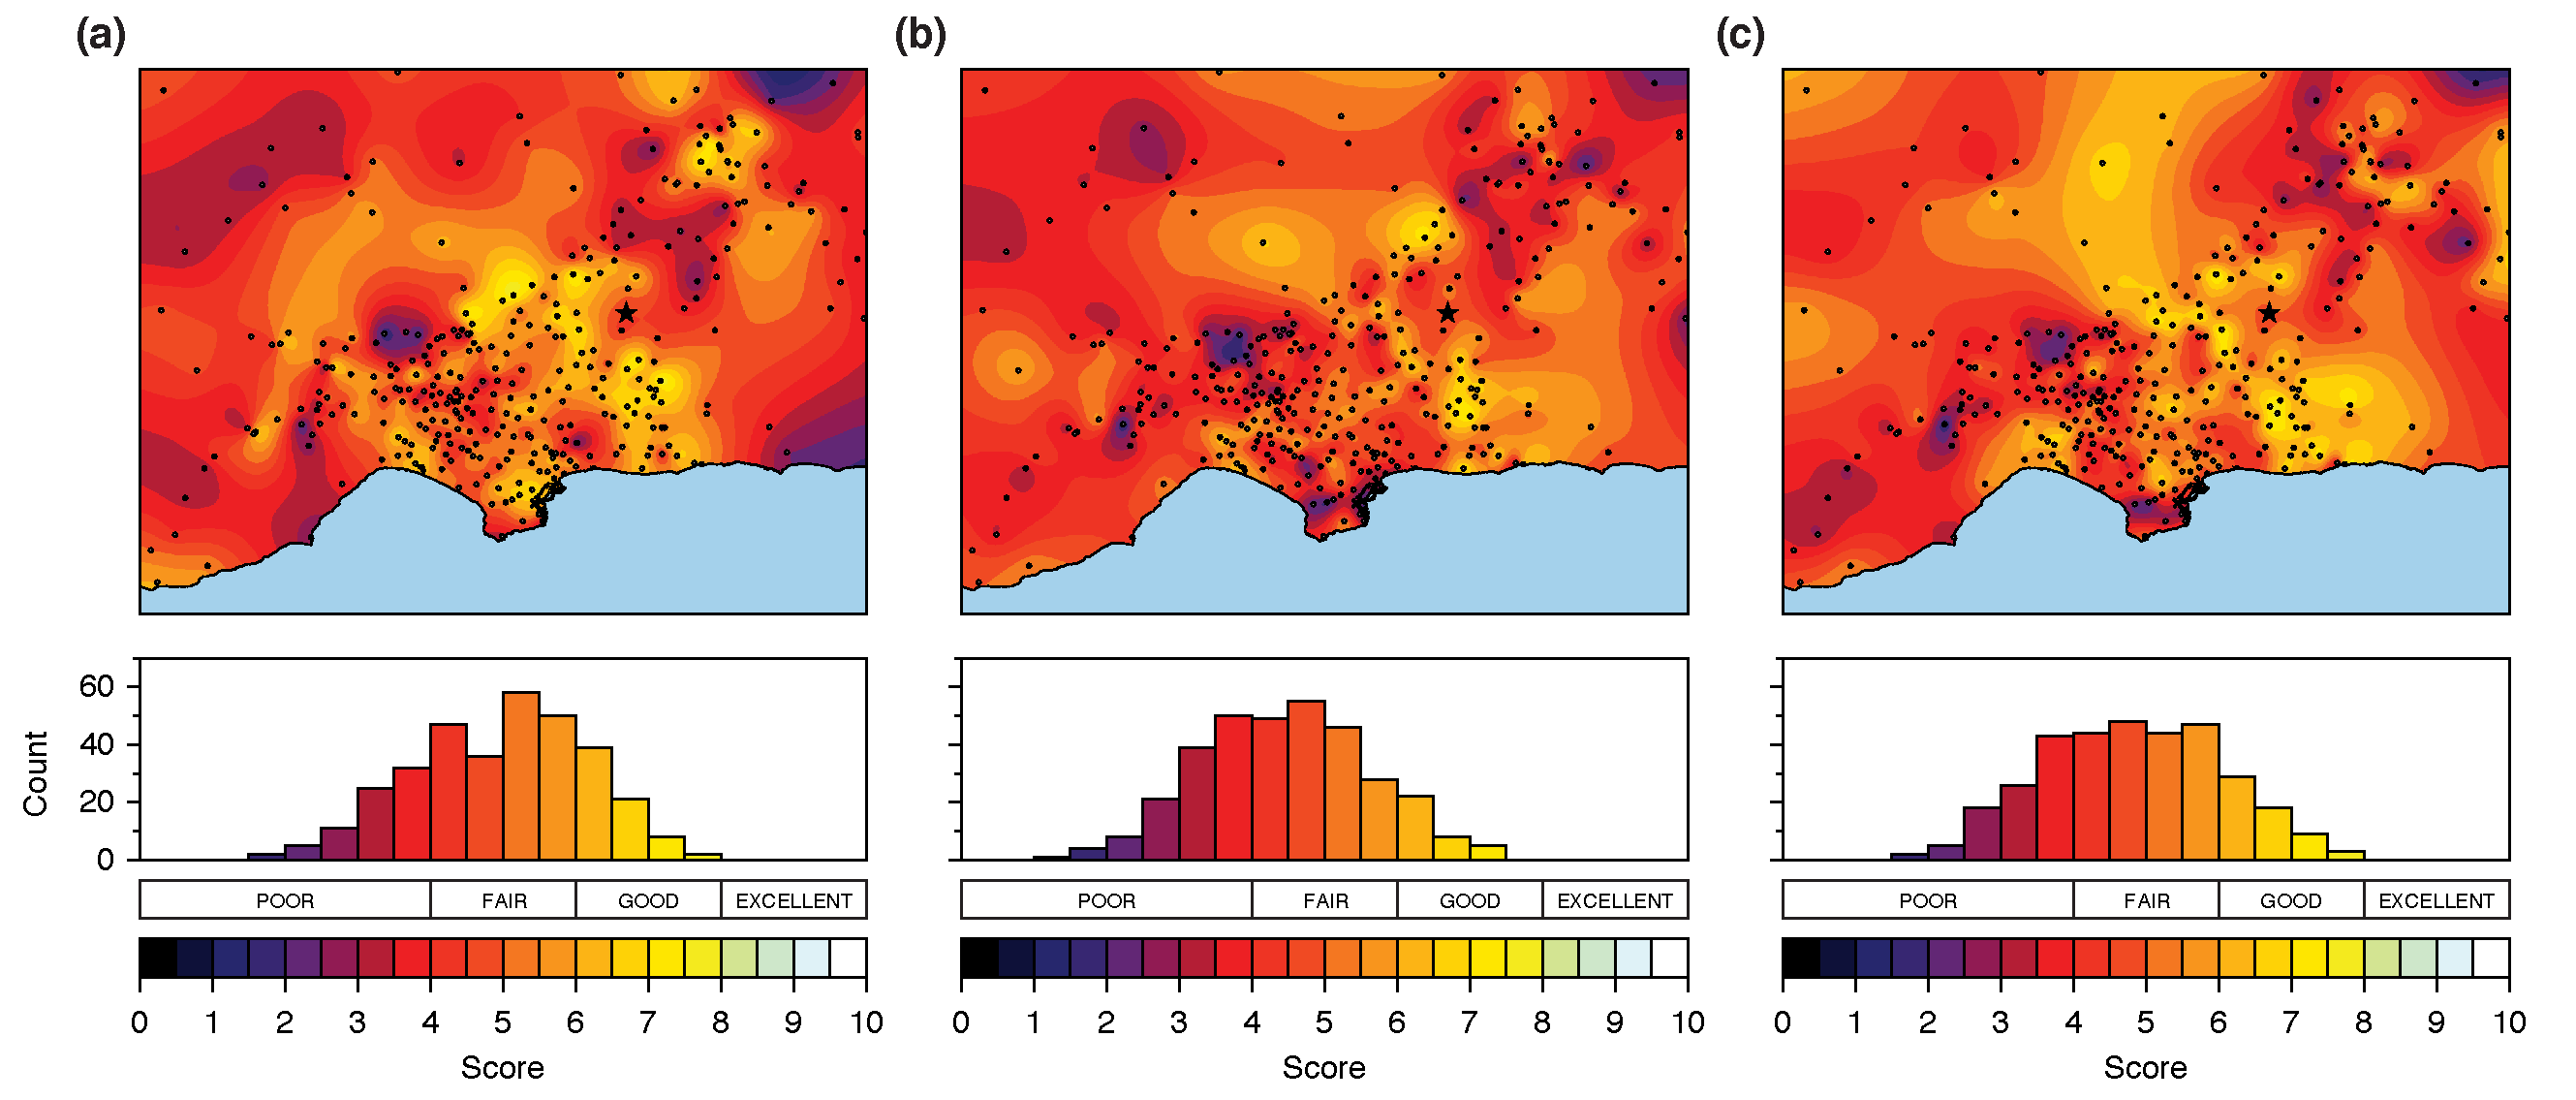
\includegraphics[width=\textwidth]{figures/pdf/figure-02}
    \caption{Validation results obtained by \citet{Taborda_2014_BSSA} in the form of GOF values across the region of interest obtained from comparisons between simulations for three different velocity models and data recorded at ground motion monitoring stations. The color version of this figure is available only in the electronic edition.}
    \label{fig:ref-gof-maps}
\end{figure*}
% 
\begin{figure}[ht!]
    \centering
    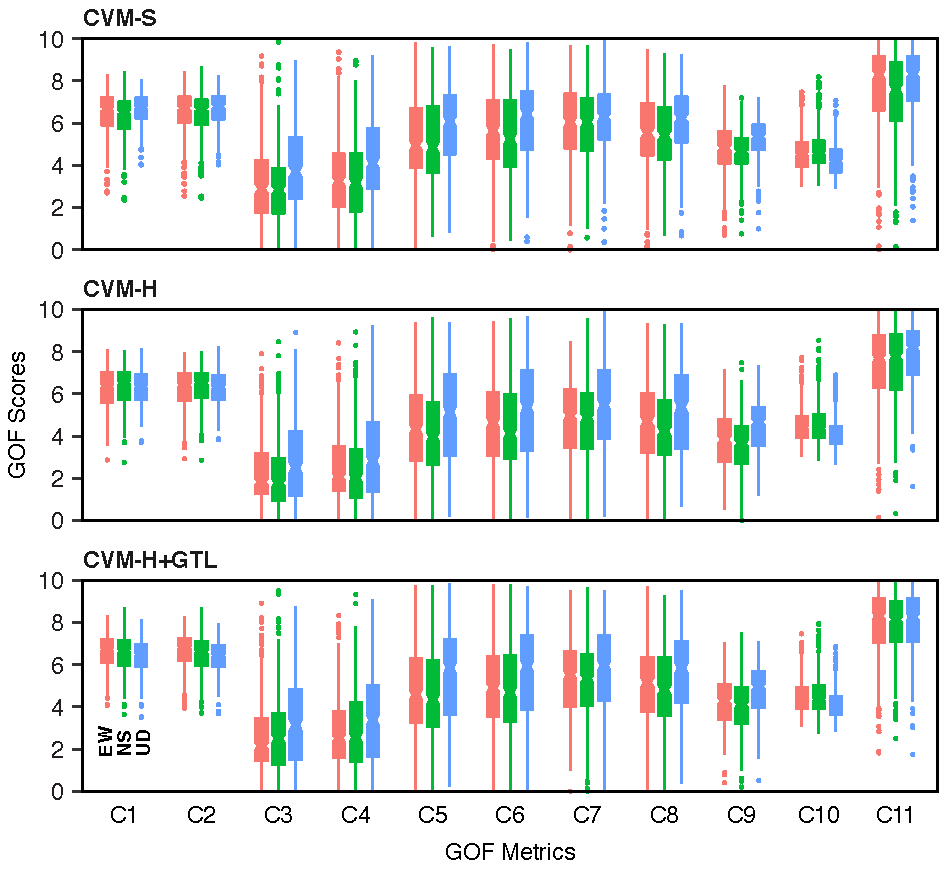
\includegraphics[width=0.48\textwidth]{figures/pdf/figure-03}
    \caption{Statistical distribution of the GOF dataset obtained from \citet{Taborda_2014_BSSA} shown in the form of box-plots for each metric (C1 through C11, see Table \ref{tab:metrics}), velocity model (CVM-S, CVM-H, and CVM-H+GTL), and component of motion (NS, EW, UD). In each case, the median is indicated by a notch in the box, the boxes represents the interquartile range ($\mathrm{IQR} = \mathrm{Q}3 - \mathrm{Q}1$), and the line shows the range of the data, with outliers (data less than $\mathrm{Q}1 - 1.5 \mathrm{IQR}$ and greater than $\mathrm{Q}3 + 1.5 \mathrm{IQR}$) shown as scattered dots. The color version of this figure is available only in the electronic edition.}
    \label{fig:data-box-plot}
\end{figure}

Here, we use the GOF scores obtained by \citet{Taborda_2014_BSSA} independently of the velocity models and/or the component of motions. Although at times we will make distinctions between the models and the components for visualization purposes, the clustering analysis to be described in the following section was done using the whole dataset of scores. The motivation behind this choice was that the dataset, as a sample of GOF values, was independent of the simulation and serves here as a generic set for the purpose of identifying the correlations that exist between the different metrics in Table \ref{tab:metrics}. As such, given the simulations for each velocity model (3), the motion components (3), and the number of stations used in the validation (336) gave us a large enough sample of 3,024 GOF scores. Figure \ref{fig:data-box-plot} illustrates this idea by comparing the statistical distribution of the broadband GOF scores of the simulations classified by velocity models and components. It is clear that although there are differences between them, these are negligible; in other words, the statistical distribution of results for each metric is about the same independently of model or component. Consequently, we combine all the data into a single dataset.



\section{Data Analysis Method} 
\label{sec:method}

We are interested in proposing an algorithm with a reduced and prioritized number of validation metrics based on previously acquired \change{collection of validation data samples} (i.e., our dataset). A common method to do this is to identify rules with disjunctive characteristics, in the form of decision trees, that lead to outcomes representative of the overall validation analysis. In our case, we define such outcome in terms of four \change{\textit{validation categories} or \textit{classes}} representative of the quality of the validation, namely: poor (P), fair (F), good (G), and excellent (E). The development of such decision trees requires a proper classification of the data, which can be done through a clustering process. \change{This this implies applying the \textit{labels} P, F, G and E to the data samples in our dataset.} The following sections explain the data processing analysis we put in place to \change{label the data samples in our} dataset and subsequently obtain \change{three} alternative decision trees.


\subsection{Clustering}
\label{sec:clustering}

The first step towards obtaining a decision tree is to label the data according to their attributes. The inherent attribute of our data are the GOF values, but because of the multiplicity of metrics and lack of clarity about their relationships, we need to label the data according to the validation categories. We do this by means of a clustering process. 

Clustering is an unsupervised data-mining process used to group data in a multi-dimensional space based on their attributes \citep{Fayyad_1996_IEEE}. According to \citet{Jain_1999_ACMCS}, clustering can be classified in two categories: hierarchical and partitional. Technical details aside, the basic difference is that hierarchical algorithms create nested partitions, whereas partitional algorithms produce singular partitions. 

There is no single clustering process that can be applied to every dataset \citep{Dy_2004_MLR, Jain_1988_Book, Hartigan_1985_JOC}. Consequently, one needs to make choices. We use a partitional, distance-based method known as constrained \kmeans{}. The standard \kmeans{} method is a process for partitioning a $n$-dimensional population into $k$ clusters with a minimum within-cluster attributes variance \citep[e.g.,][]{Macqueen_1967_Proc}. Constrained \kmeans{} extends this method by allowing the use of background information in the form of clustering restrictions.

Given a $k$ number of clusters, where each cluster is identified by its center, the standard process starts by computing the distances of all other data-points to the center of the clusters, and grouping them based on their proximity to the clusters' centers. Once this is done, the center of each cluster is updated based on the average attributes of its data-points, and the process is repeated until the clusters become stable.

\begin{figure}[ht!]
	\centering
	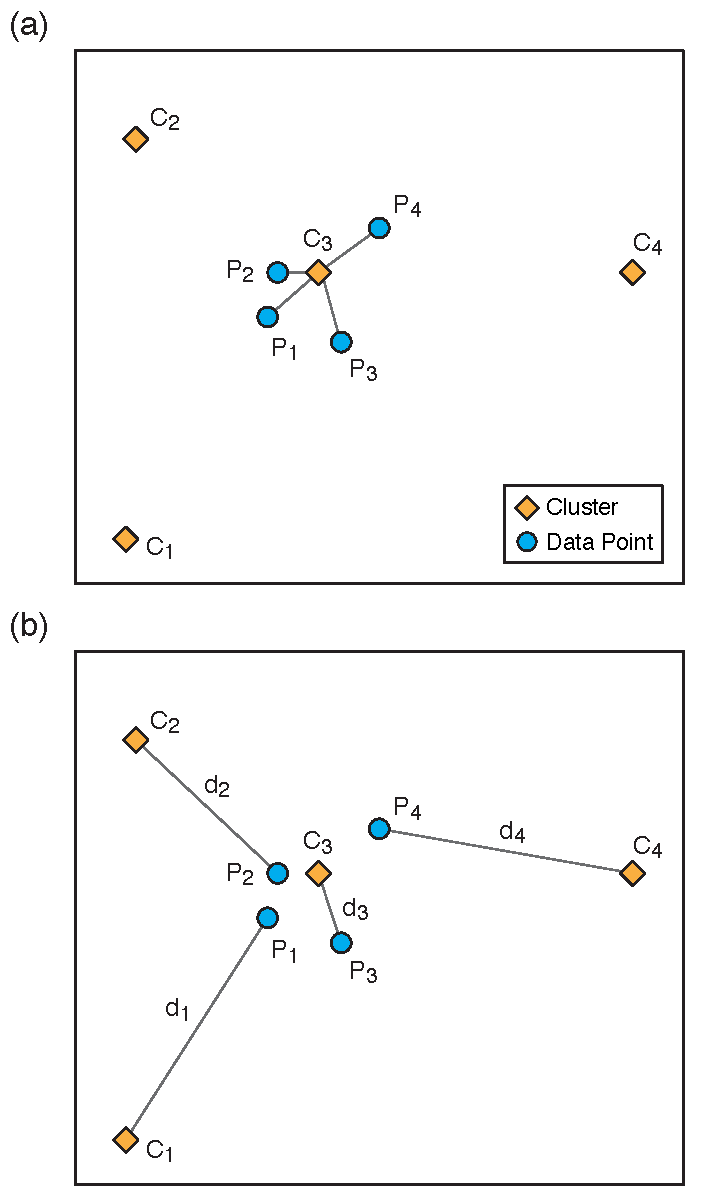
\includegraphics[width=\columnwidth]{figures/pdf/figure-04}
	\caption{Representation of the (a) ordinary, and (b) constrained \kmeans{} approaches for four data-points (P) and four cluster centers (C) in a 2D dataset space, where all the data-points are constrained to be cannot-link points. The color version of this figure is available only in the electronic edition.}
	\label{fig:k-means}
\end{figure}

This process is sensitive to the initial selection of the clusters and their centers. To mitigate this, constrained \kmeans{} introduces two types of constraints: must-link and cannot-link \citep{Wagstaff_2001_Proc}. The must-link constraint specifies instances in which two data-points must be linked, i.e., in the same cluster. The cannot-link constraint specifies instances in which data cannot be in the same cluster. This prevents the process from converging into a local minimum, and defines constrained \kmeans{} as a semi-supervised method. Figure \ref{fig:k-means} illustrates the differences between the standard and constrained \kmeans{} methods for a single clustering iteration on a small two-dimensional dataset.

In our implementation we limit the clustering to four validation categories: poor, fair, good, and excellent. The cluster centers are randomly selected at the start, but we apply constraints by adding 4 artificial stations with cannot-link conditions that are checked at the end of each iteration. These stations are associated with each type of cluster and have GOF scores equal to 3, 5, 7, and 9, across all metrics, thus they are representative of the validation categories. 

In the multi-dimensional space defined by the 11 GOF metrics used here, the distances are obtained using the Euclidean expression:
% 
\begin{equation}
	d(x_i, x_j) = \sqrt{ \sum_{l=1}^{n} \left( x_{i,l} - x_{j,l} \right)^2 } 
\end{equation}
% 
corresponding to the distance $d$ between the data-point $x_i$ and the cluster center $x_j$ in the $n$-dimensional domain, where $x_{i,l}$ is the $l$-th feature of the data-point $x_i$, and $x_{j,l}$ is the $l$-th feature of the cluster center $x_j$. It is, however, unpractical to expect the patterns defining the clusters to be observable across all features. Such high-dimensional issues are well known \citep[see, for instance,][]{Parsons_2004_ACM, Dy_2004_MLR}, and can be tackled using sub-spaces. Therefore, instead of analyzing all $2^{11}$ possible sub-spaces, we focus only on sub-spaces with 2, 3, and 4 dimensions, or features. In total, we analyze 550 sub-spaces, 55 sub-spaces with 2 features, 165 with 3, and 330 with 4.

Unfortunately, not all the sub-spaces will have clearly distinguishable clusters (i.e., some will not satisfy the cannot-link constraints even after a large number of iterations). Such sub-spaces are discarded, and all others are used to label the data. In an ideal case, each station will be labeled 550 times, and the final label is taken as the mode. For example, if after all the sub-spaces are accounted for, a station has labels $\left\{F, F, F, P, F, G, E, F, F\right\}$, where the labels $P$, $F$, $G$, and $E$ correspond to the poor, fair, good, and excellent category clusters, then such as station will be given a final label $F$. Once all the data is properly labeled, we proceed with the decision tree analysis.


% ===========================================================================================
%


% Although we do not expect to see the pattern that resulted from clustering using 11 features in presentation of only two, however, different studies show that the higher dimension reduce the effect of similarity based on distance. \citet{Parsons_2004_ACM} presented an illustrative example to show the effect of dimension in reducing the importance of the distance. Effect of higher dimensions in clustering has been well studied and many different methods are proposed to reduce this effect in the final results. Among them we can name  feature selection before, during, and after clustering, hybrid methods that use combination of methods to select the best subset of feature. \citet{Dy_2004_MLR} addressed two issues involved in developing an automated feature subset selection algorithm for unlabeled data. They illustrated the irrelevant and redundant features and proposed methods for evaluating candidate features using two performance criteria.

% Subspace analysis is another technique to address the challenges with higher dimensional data in clustering process. Subspace clustering is an extension of traditional clustering which looks for different pattern using subset of features.  \citet{Parsons_2004_ACM} provided a list of algorithm for conducting subspace clustering and also some potential applications for them. The most common factor among these algorithm is the process to find a group of best subspaces through optimization process. An n-dimensional dataset has $2^n$ subspaces where it could be very costly and time consuming to evaluate all of them.

% In this study we are interested in using those features who, in general, represent the simulation accuracy in 4 different categories. As a first step we use the constrained \kmeans{} clustering approach for all features, however, because of mentioned reasons the results are not easy to discuss or even evaluate. Although we have four groups of data, the question is which one should be considered as poor, fair, good, or excellent groups. Therefore, we apply a modified method of subspace clustering approach to cluster the stations. As we discussed earlier and presented in figures the constrained \kmeans{} method effectively put the stations in a cluster with considering the fact that our constrain stations should not be in the same cluster. High number of iteration leads the clustering process to follow the clustering concept that we are looking for which is clustering stations as poor, fair, good, and excellent. In our case number of possible subspace is $2^{11}$ where each features have two options wether belong to subspace or not. However, because of preserving the distance based criteria effects we limited the number of features in the subspace to be 2,3, and 4 features. Therefor we have 330,165, and 55 unique subspaces for 4D,3D, and 2D, respectively. We conduct a constrained \kmeans{} clustering analysis for each of these subspaces and repeat the algorithm. In some cases, it is not possible to distinguish all four cannot-link stations in different clusters. In this study we ignore these cases. We only use those combination of features that gives 4 unique clusters for the constraint points (hypothetical stations), therefore, we know for sure that all data within same cluster let's say with metric value 3, should be considered as poor. We also control the clusters to be consistent (we reformat numbers to assign cluster 1 to all group of stations that our first constraint belongs to them and so on). Finally, using 550 unique subspace clustering results, we assign the most frequent class to the station.





% and computes . These distances are then used as a criteria to determine the cluster to which cluster each data-point belongs. 

% ...


% \citet{Macqueen_1967_Proc} describes this method as a process for partitioning a $n$-dimensional population into $k$ sets on the basis of a sample. Its algorithm produces partitions that are reasonably efficient in the sense of within-class variance. It starts with a user defined number of clusters ($k$) and assigns a random mean value to each cluster (or randomly choose $k$ data-points and assigns them as cluster centers). After this, the algorithm computes the distances of all other data-points to the center of the cluster and uses the distance as a criteria to clustering the data points. Because the data resides in a multi-dimensional space (here defined by each metric), there are different ways of computing the distance of each data-point to the cluster's center. We use the Euclidean distance:
% % 
% \begin{equation}
% 	d(x_i, x_j) = \sqrt{ \sum_{k=1}^{n} \left( x_{i,k} - x_{j,k} \right)^2 } 
% 	\, ,
% \end{equation}
% % 
% where $n$ is the number of features and $d$ is the distance of $x_i$ and $x_j$ in $n$-$dimensional$ domain. 




% ===========================================================================================
%
% NEW TEXT PROVIDED BY NAEEM ON JAN 22
% Once the distance is computed, the algorithms labels the data based on the proximity of each point to each cluster, and computes the arithmetic mean value of the data for each cluster, and assigne that value as the updated location of each cluster's center. The algorithm repeats the steps unless the amount of updates among the cluster centers is less than a predefined tolerance value. The major problem with \kmeans{} algorithm is that it is sensitive to the selection of the initial partition and may converge to a local minimum of the criterion function value if the initial partition is not properly chosen. Another problem accompanying the use of \kmeans{} algorithm is the choice of the number of desired output clusters. \citep{Jain_1999_ACMCS}. Clustering is a subjective process. The same set of data items often needs to be partitioned differently for different application. In our application the number of clusters according to the literature is 4 (i.e., poor, fair, good, and excellent.) However, our initial attempts represents that the results are highly sensitive to the initial clusters' center. Therefore, we need to incorporate the experts knowlege in the process. 


% \citet{Wagstaff_2001_Proc}  demonstrated a modification of \kmeans{} clustering algorithm which uses the background information of the domain or dataset. The algorithm adds two types of constraints to the clustering including:
% 	% 
% 	\begin{itemize}
% 	\item{Must-link: constraints specify that two instances have to be in the same cluster.}
% 	\item{Cannot-link: constraints specify that two instance must not be placed in the same cluster.}
% 	\end{itemize} 
% 	% 
% The algorithm is described in detail in \citet{Wagstaff_2001_Proc}, however, in simple words, in the ordinary \kmeans{} process before assigning data to the closes cluster, it controls the must-link and cannot-link conditions. Therefore, in this case, the closest cluster's center is not necessarily the final cluster of the data.


% In a hypothetical assumption, if we have a pair of data and synthetic with GOF score of 3 for all metrics we could consider the overall simulation GOF as poor. This is also correct for 5,7, and 9 that we can assigne them fair, good, and excellent class, respectively. Therefore, we add 4 hypothetical stations into the dataset with GOF score of 3,5,7,and 9 for all metrics and we put them in cannot-link constraint. This assumption that originated from the experts knowledge, provides enough information to the algorithm to converge to the same final clusters and cluster centers after a reasonable amount of iteration. 

% Fig.~\ref{fig:con_kmeans} presents the difference between ordinary and constrained k-means clustering approach using 4 points and 4 cluster centers. Fig.~\ref{fig:con_kmeans}.a presents the \kmeans{} without constrained. According to the definition and the explanation in this section, the closest cluster center for each points will get the points. 	Fig.~\ref{fig:con_kmeans}.b represents the constrained \kmeans{} approach, where, the closest cluster center is not necessarily the final cluster. The data points can not be in the same cluster, in result,  we assign them to different clusters in this case to satisfy the Cannot-link criteria. The best configuration happens when we minimize the distance between cluster centers and points.

% ===========================================================================================
% 
% OLD STUFF DONE BY RICARDO FOR THE INTRO OF THIS SECTION
% 
% In machine learning, decision trees are classified as a supervised learning method, and the first step towards designing them requires that the data be labeled according to their attributes. The inherent attribute of our data are the GOF value themselves, but because of the multiplicity of metrics and the lack of clarity about how these relate to each other, we need to add labels to the data that are in accordance with the outcome attributes, i.e., in terms of the predefined validation quality levels. We label the data in our dataset by means of a clustering process. 

% There exist different methods for clustering data \citep[see Chapters 10 and 11 in][]{Han_2011_Book}, among which the \kmeans{} and constrained \kmeans{} clustering methods are the most widely used \citep{Jain_1999_ACMCS}. We note about these methods that the \kmeans{} approach is sensitive to the initial values chosen to be at the center of the clusters---especially in the case of data that are not clearly distinguishable---, whereas the constrained \kmeans{} method uses background knowledge to overcome this limitation. Because of its use of background information, the modified \kmeans{} method is considered as a semi-supervised process.





% ===========================================================================================
%
% SECOND ATTEMPT THAT WAS RECALLED BY NAEEM

% Once the distance is computed, the algorithms labels the data based on the proximity of each point to each cluster, computes the mean value of the data for each cluster, and updates the location of each cluster's center. \textcolor{red}{(How do we compute ``mean value'' and how do we recompute the ``center''? All what follows after this in the original text is too descriptive, and not specific enough. We need to go to the point and this is going in long description circles.)} 

% {\color{gray}
% 	The algorithm repeats the steps unless the amount of updates among the cluster centers is less than a tolerance value.  \kmeans{} clustering has been applied in different applications, however, there is no clustering technique that is universally applicable in uncovering the variety of structures present in multidimensional datasets. Therefore, clustering is a subjective process. The same set of data items often needs to be partitioned differently for different application. In result, it is essential for the user of a clustering algorithm to not only have a thorough understanding of the particular technique being utilized, but also to know the details of the data gathering process and to have some domain expertise; the more information the user has about the data at hand, the more likely the algorithm would be able to succeed in assessing its true class structure. Domain concept can play several roles in the clustering process, and a variety of choices are available to the practitioner \citep{Jain_1999_ACMCS}. 

% 	The major problem with \kmeans{} algorithm is that it is sensitive to the selection of the initial partition and may converge to a local minimum of the criterion function value if the initial partition is not properly chosen. Another problem accompanying the use of \kmeans{} algorithm is the choice of the number of desired output clusters. Several variant of the \kmeans{} algorithm have been reported in the literature. Some of them attempt to select a good initial partition so that the algorithm is more likely to find the global minimum value, another variation is to permit splitting and merging of the resulting clusters \citep{Jain_1999_ACMCS}. 

% 	In our application the number of clusters is not a problem and there is a consensus among researchers in the number of clusters (i.e., poor, fair, good, excellent), however, our initial attempts represent that the results are highly sensitive to the initial clusters' center. 

% 	Every clustering algorithm uses some type of knowledge either implicitly or explicitly. In this study the background knowledge is a series of hypothetical stations. We assume that there are four stations with score of 3, 5, 7, and 9 for all of their metrics. Based on the score limits in section.~\ref{validation_metrics} we know these stations belong to poor, fair, good, and excellent classes, respectively. These background knowledge could help the clustering processing to be in right direction regarding the fact that increasing dimension of data could increase noise in clustering and cause difficulty to better partitioning. \citet{Wagstaff_2001_Proc}  demonstrated a modification of \kmeans{} clustering algorithm which uses the background information of the domain or dataset. The algorithm adds two types of constraints to the clustering including:
% 	% 
% 	\begin{itemize}
% 	\item{Must-link: constraints specify that two instances have to be in the same cluster.}
% 	\item{Cannot-link: constraints specify that two instance must not be placed in the same cluster.}
% 	\end{itemize} 
% 	% 
% 	The algorithm is described in detail in \citet{Wagstaff_2001_Proc}, however, in simple words, in the ordinary \kmeans{} process before assigning data to the closes cluster, it controls the must-link and cannot-link conditions. Therefore, in this case, the closest cluster's center is not necessarily the final cluster of the data. Fig.~\ref{fig:con_kmeans} presents the difference between ordinary and constrained k-means clustering approach using 4 points and 4 cluster centers. Fig.~\ref{fig:con_kmeans}.a presents the \kmeans{} without constrained. According to the definition and the explanation in this section, the closest cluster center for each points will get the points.
	
% 	Fig.~\ref{fig:con_kmeans}.b represents the constrained \kmeans{} approach, where, the closest cluster center is not necessarily the final cluster. The data points can not be in the same cluster, in result,  we assign them to different clusters in this case to satisfy the Cannot-link criteria. The best configuration happens when we minimize the distance between cluster centers and points. Using this method at each step the algorithm redistribute the 4 hypothetical stations to satisfy the cannot-link constraint. The visual inspection of the figures also confirms the accuracy of the method. Doing this, in the next iteration this data manipulation leads the cluster center in a direction to have the hypothetical station in the cluster and loose those data that is in far other side direction of the hypothetical station. Therefore, the cluster tend to have all data that similar to the hypothetical station. \\
% 	The end product of the clustering process is groups of data. Analysis of these groups, individually, gives the idea about the clusters in terms of within class variation. In these analysis we mainly study the behavior of different features in each cluster and isolate only the most descriptive features to be used in the supervised classifier that assumes a given number of classes in the data set. In the next section we provide a basics of decision tree algorithm. 

% }

% In other words, the points cannot be in the same cluster. In the constrained \kmeans{} approach we redistribute the points such that the $\sum{d}$ becomes minimum.

% ===========================================================================================
%
% OLD NAEEM VERSION
% 
% Clustering is an unsupervised approach for grouping of data based on measure of similarity and it is considered as an exploratory activity as a part of data mining process \citep{Fayyad_1996_IEEE}. In each valid cluster, patterns are more similar in each other than they are to pattern belonging to a different cluster. Many clustering algorithms are developed for different application, however, study the difference of them is beyond the scope of this paper. In general, at the top level,  \citet{Jain_1999} distinguished the clustering approach into Hierarchical and Partitional approaches. Aside from differences in application and technical details in implementation, hierarchical methods produce nested series of partitions, while partitional methods produce only one. In this study we are interested in using partitional, distance based clustering algorithm, which is also known as \kmeans{} algorithm.  \citet{Macqueen_1967_Proc}  described a process for partitioning an $n$-$dimensional$ population into $k$ sets on the basis of a sample. The process appears to give partitions which are reasonably efficient in the sense of within-class variance. For numerical values, \kmeans{} algorithm starts with a user defined number of clusters (k) and assign a random mean value for each cluster (or randomly choose k data and assign them as cluster centers.) Then it computes the distance of data and cluster centers. A variety of distance measures are in use in different studies, however, we use the Euclidean distance through 

% \begin{equation}
% d(x_i,x_j)=\sqrt{\Sigma_{k=1}^{n}(x_{i,k} - x_{j,k})^2},
% \end{equation}

% where $n$ is the number of features and $d$ is the distance of $x_i$ and $x_j$ in $n$-$dimensional$ domain. After computing the distance of the points from each clusters' mean (center), the algorithm continues with labeling the data after the closest cluster. At the next iteration, it computes the mean value of data for each cluster and updates the clusters' centers. The algorithm repeats the steps unless the amount of updates among the cluster centers is less than a tolerance value.  \kmeans{} clustering has been applied in different applications, however, there is no clustering technique that is universally applicable in uncovering the variety of structures present in multidimensional datasets. Therefore, clustering is a subjective process. The same set of data items often needs to be partitioned differently for different application. In result, it is essential for the user of a clustering algorithm to not only have a thorough understanding of the particular technique being utilized, but also to know the details of the data gathering process and to have some domain expertise; the more information the user has about the data at hand, the more likely the algorithm would be able to succeed in assessing its true class structure. Domain concept can play several roles in the clustering process, and a variety of choices are available to the practitioner \citep{Jain_1999}. 

% The major problem with \kmeans{} algorithm is that it is sensitive to the selection of the initial partition and may converge to a local minimum of the criterion function value if the initial partition is not properly chosen. Another problem accompanying the use of \kmeans{} algorithm is the choice of the number of desired output clusters. Several variant of the \kmeans{} algorithm have been reported in the literature. Some of them attempt to select a good initial partition so that the algorithm is more likely to find the global minimum value, another variation is to permit splitting and merging of the resulting clusters \citep{Jain_1999}. 

% In our application the number of clusters is not a problem and there is a consensus among researchers in the number of clusters (i.e., poor, fair, good, excellent), however, our initial attempts represent that the results are highly sensitive to the initial clusters' center. 

% Every clustering algorithm uses some type of knowledge either implicitly or explicitly. In this study the background knowledge is a series of hypothetical stations. We assume that there are four stations with score of 3, 5, 7, and 9 for all of their metrics. Based on the score limits in section.~\ref{validation_metrics} we know these stations belong to poor, fair, good, and excellent classes, respectively. These background knowledge could help the clustering processing to be in right direction regarding the fact that increasing dimension of data could increase noise in clustering and cause difficulty to better partitioning. \citet{Wagstaff_2001_Proc}  demonstrated a modification of \kmeans{} clustering algorithm which uses the background information of the domain or dataset. The algorithm adds two types of constraints to the clustering including:\\
% \begin{itemize}
% \item{Must-link: constraints specify that two instances have to be in the same cluster.}
% \item{Cannot-link: constraints specify that two instance must not be placed in the same cluster.}
% \end{itemize} 
% The algorithm is described in detail in \citet{Wagstaff_2001_Proc}, however, in simple words, in the ordinary \kmeans{} process before assigning data to the closes cluster, it controls the must-link and cannot-link conditions. Therefore, in this case, the closest cluster's center is not necessarily the final cluster of the data. Fig.~\ref{fig:con_kmeans} presents the difference between ordinary and constrained k-means clustering approach using 4 points and 4 cluster centers. Fig.~\ref{fig:con_kmeans}.a presents the \kmeans{} without constrained. According to the definition and the explanation in this section, the closest cluster center for each points will get the points.
% Fig.~\ref{fig:con_kmeans}.b represents the constrained \kmeans{} approach, where, the closest cluster center is not necessarily the final cluster. The data points can not be in the same cluster, in result,  we assign them to different clusters in this case to satisfy the Cannot-link criteria. The best configuration happens when we minimize the distance between cluster centers and points. Using this method at each step the algorithm redistribute the 4 hypothetical stations to satisfy the cannot-link constraint. The visual inspection of the figures also confirms the accuracy of the method. Doing this, in the next iteration this data manipulation leads the cluster center in a direction to have the hypothetical station in the cluster and loose those data that is in far other side direction of the hypothetical station. Therefore, the cluster tend to have all data that similar to the hypothetical station. \\
% The end product of the clustering process is groups of data. Analysis of these groups, individually, gives the idea about the clusters in terms of within class variation. In these analysis we mainly study the behavior of different features in each cluster and isolate only the most descriptive features to be used in the supervised classifier that assumes a given number of classes in the data set. In the next section we provide a basics of decision tree algorithm. 


% \begin{figure}
%     \centering
%     \includegraphics
%       %  [width=\columnwidth]
%         [width=200px]
%         {figures/pdf/Figure_4.pdf}
%     \caption{ Representation of ordinary (a) and constrained (b) \kmeans{} approach. There are four data points (p) and four cluster centers (c) as a sample of $2$-$Dimensional$ dataset. All points are defined as cannot-link constraints. In other words, the points cannot be in the same cluster. In the constrained \kmeans{} approach we redistribute the points such that the $\sum{d}$ becomes minimum.}
%     \label{fig:con_kmeans}
% \end{figure}




\subsection{Decision Trees}
\label{sec:decision-tree}

Building decision trees is a supervised learning process used to approximate a target function as a sequence of disjunctive conditions designed to measure the effectiveness of a set of attributes to classify data and predict outcomes. The theory behind decision trees is well established \citep[e.g.,][]{Quinlan_1986_ML, Mitchell_1997_Book}. 
\myrevision{A decision tree can be used to classify a case by starting at the root of the tree and moving through it until the leaf is encountered. Each tree is a structure including a root, decision nodes and leaf nodes. Decision nodes specifies some test to carried out on attributes and leaf nodes indicate the final class \citep{Quinlan_1993_Book}.} Decision trees are, however, non-unique. They depend on the dataset, the user parameters, and the algorithm employed to build them \citep{Murthy_1998_DMKD}. Therefore, before describing our choice of the decision tree algorithm and parameters, we revise three aspects about the dataset: data classes, attributes equivalence, and dataset balance.

First, regarding data classes we refer to whether the classes of data are properly distinguishable or not, and to whether the data attributes contribute to those classes or not. In our case, data classes are handled by means of the clustering and labeling process. As we described in the previous section, at the end of the clustering process, all the data-points (or samples) in our dataset get labeled with one out of four outcome classes (or clusters) defined in terms of the validation categories (poor, fair, good, excellent).

Second, attributes equivalence refers to whether the data attributes are comparable with each other on equivalent terms or not. There are cases, either because of the method or because of the data, that the data attributes need to be standardized. In artificial neural networks, for instance, the data needs to be normalized on a $[-1,1]$ or $[0,1]$ scale. Normalization is also necessary when data attributes come in different unit scales or value ranges \citep[e.g.,][]{Wu_2010_JH}. In our case, this is not necessary because (a) all the data attributes---defined by the 11 GOF metrics---are on the same dimensionless numerical scale (varying from 0 to 10), and (b) because the algorithm we use is not susceptible to the attributes scale.

Last, there is the issue of balance. A balanced dataset is one that has about the same number of samples per class. Algorithms used for building decision trees tend to perform better with balanced datasets \citep[e.g.,][]{Branco_2016_ACMCS, Weiss_2003_JAIR}. Imbalanced datasets, on the other hand, are those with a significant disparity in the number of samples in each class. Imbalanced datasets can be improved by a resampling process. There are two basic resampling approaches: undersampling and oversampling \citep{Branco_2016_ACMCS}. Undersampling discards data from the subsets with larger number of samples. Oversampling replicates data until reaching appropriate number of samples. Both processes are done by randomly picking data to either be discarded or replicated. In our case, as we will see later, we apply oversampling to one of our dataset classes. This process has consequences, mainly that it increases the likelihood of overfitting. \myremove{A matter we discuss later.} \myrevision{Overfitting happens when the prediction algorithm predicts the final results too closely or exactly to the training data, however, it provides non-accurate results for unseen or test data.}

Upon completing the clustering and resampling processes, the next step is to subdivide the dataset in two, a training dataset (with 70 percent of the samples picked randomly), and a testing dataset (with the remaining 30 percent). We first use the training dataset to build a large suite of potential decision trees, and then use the testing dataset to evaluate and pick the best possible decision tree(s) among them. There are several algorithms for building decision trees \citep[e.g., ID3, C4.5, C5.0, CART; see][]{Quinlan_1986_ML, Quinlan_1993_Book, Quinlan_1996_JAIR, Breiman_1984_Book}. \myrevision{C5.0 is considered as the developed version of ID3 and C4.5, where it does not have any limitations in handling missing data, numerical attributes, and developing boosted models. Internal algorithm of CART is different than other methods, however, discussing technical details of these algorithms are beyond the scope of this study.} Here we use the C5.0 implementation \citep{Kuhn_2017_Manual}, which is an extension of the C4.5 algorithm developed by \citet{Quinlan_1993_Book, Quinlan_1996_JAIR}.

In essence, given a dataset, the process of building the tree consists of recursively identifying the attributes in the training data that are most likely to predict an outcome. The process is recursive because new branches and decision nodes are created based on the remaining data at every branch and level, until the tree reaches a certain depth or when other conditions are met. The effectiveness of an attribute $A$ in classifying any subset $S$ from the training data is measured through the information gain $G$ as
% 
\begin{equation}
	\label{eq:gain}
	G(S,A) = E(S) - \sum_{v \, \in \, A[a]} \frac{ \left| S_v \right| }{ \left| S \right| } E \left( S_v \right)
	\, ,
\end{equation} 
% 
where $A[a]$ is the set of all possible values of attribute $A$, $S_v$ is the subset of $S$ for which attribute $A$ has value $v$, and $E(\cdot)$ is the entropy function given by
% 
\begin{equation}
	E(S) = \sum_{i=1}^{c} \Big( -p_i \log_2 \left(p_i\right) \Big)
	\, ,
\end{equation}
% 
where $p_i$ is the proportion of $S$ belonging to class $i$, and $c$ are the different values that a given target attribute can take.

Entropy measures the homogeneity of a set of data. The higher the entropy, the more even the distribution of the data across classes. Conversely, an extremely low value of entropy would mean most of the data falls within a particular class. With this in mind, the information gain $G$ of an attribute $A$ for the dataset $S$, or $G(S,A)$ in equation (\ref{eq:gain}), is the expected reduction in entropy caused by partitioning the dataset according to attribute $A$ \citep{Mitchell_1997_Book}. For selection of a threshold for a \myrevision{numerical} continuous attribute refer to \citet{Quinlan_1996_JAIR}.

In the particular case of the C5.0 algorithm the result of this process depends on several parameters, logical and numerical. We set the options to do feature selection \myrevision{or winnowing. Therefore, the algorithm choose to use the most important attributes and ignore others. We also activate the evaluation of possible advanced splits of data. Sometimes data is very close to the splitting threshold where assigning a hard threshold may incorrectly change the classification, whereas, that small difference could happen because of numerical errors or error in measurement. Therefore, advanced split can define a soft threshold to consider different probabilities in assigning data to different classes. A decision tree can grow so deep to finally classify all training data correctly. However, the tree will be very complex and will suffer from overfitting. In other words it will have very poor functionality for test data. Therefore, decision tree algorithms (here C5.0) first grow the tree up to the most complex tree then based on user defined factors start to prune the grown tree.The pruning process helps to reduce the complexity of the tree and also increase it's generalizability. Consequently the pruned tree's leaf nodes will have training data which belongs to more than one class which the final class will be the mode of that leaf node. In this study we use two parameters to control the pruning process including confidence or certainty factor (CF) and the smallest number of samples that must be put in at least two of the splits ($S_{\min}$, also known as \textit{minCases}). C5.0 algorithm uses error-based pruning method (see \citet{Quinlan_1993_Book} for more details). The objective is to minimize the observed error rate. Therefore, error estimates for leaf nodes and subtrees are computed assuming that they were used to classify a set of unseen cases with a predicted error rate which is computed based on CF and binomial distribution of number of misclassified events (E) and all training data at that leaf (N). Decreasing CF and increasing $S_{\min}$ cause more heavy pruning process \citep[see][]{Kuhn_2017_Manual}.} \myremove{and evaluate possible advanced splits of data, but do not use the boosted models option \citep[see][]{Kuhn_2017_Manual}; and use the confidence factor (CF) and the smallest number of samples that must be placed in at least two of the splits ($S_{\min}$, also known as \textit{minCases}) to fine tune the prediction models.} In particular, we build a suite of trees for varying values of CF and $S_{\min}$.



Each tree resulting from this process has different qualities. We are interested in selecting a tree that is highly effective, but with a low level of complexity. In other words, we seek a tree with a good ratio of accuracy for predicting the classification outcome of the data, while using a reduced number of attributes (GOF metrics) in only a few number of steps (as given by a small number of decision nodes or a tree with shallow depth). The number of metrics, the number of nodes, and the depth of a tree are directly seen from the topology of the tree, and are often proportional (shallow trees tend to use less nodes, and thus less metrics). In general, smaller trees are preferable because they are easy to understand and often more accurate predictors \citep{Quinlan_1996_JAIR}.

The effectiveness of the tree, on the other hand, needs to be measured. To that end we use the factor $F_{\beta}$ proposed by \citet{Rijsbergen_1979_Book} as
% 
\begin{equation}
	\label{eq:f}
	F_{\beta} = \frac{ (1 + \beta^2) P R}{\beta^2 P + R}
	\, ,
\end{equation}
% 
where $P$ and $R$ are the precision and recall factors, respectively, and $\beta$ is a weighting factor between the two. $P$ measures the fraction of data samples that are correctly classified within a category, whereas $R$ measures the fraction of the data classified within that category regardless of whether it was correctly classified or not. Mathematically, they are defined as
% 
\begin{equation}
	P = \frac{ \mathrm{TP} }{ \mathrm{TP} + \mathrm{FP} } 
	\quad \mathrm{and} \quad
	R = \frac{ \mathrm{TP} }{ \mathrm{TP} + \mathrm{FN} }
	\, .
\end{equation}
% 
Here, TP, FP, and FN are the number of samples in the testing dataset considered to be true-positives, false-positives, and false-negatives, respectively. These values are typically ordered in what is known as a confusion matrix. For the simplest case of two categories, a confusion matrix takes the form
% 
\begin{equation}
\nonumber
\begin{array}{rr@{}rl}
	&					&	\multicolumn{2}{c}{\mathrm{Prediction}}		\\
	&					&	\mathrm{Positive}	&	\mathrm{Negative}	\\[0.75ex]
	\mathrm{Actual~Value}		
	&	\begin{array}{r}
			\mathrm{Positive} \\[1ex]
			\mathrm{Negative} 
		\end{array}
	&	\left[~
		\begin{array}{c}
			\mathrm{TP} \\[1ex]
			\mathrm{FP} 
		\end{array}\right.
	&
		\left.
		\begin{array}{cc}
			~\mathrm{FN} \\[1ex]
			~\mathrm{TN} \\[1ex]
		\end{array}~\right]
\end{array}
\end{equation}
% 
where TN is the number of true-negative samples.

We compute $F_{\beta}$ in equation (\ref{eq:f}) using $\beta = 1$ to give equal weight to $P$ and $R$ \citep{McCarthy_1995_Proc}. This is done for all the trees obtained using all possible combinations of CF and $S_{\min}$ values. Then, we select the tree with the highest level of effectiveness as \myremove{measure} \myrevision{measured} by $F_1$, commensurate to such tree having a low complexity, i.e., a reduced number of metrics and a shallow depth, which is precisely the goal set at the start. Note that $F_1$ is obtained based on the testing dataset as opposed to the training dataset. The results as applied to our dataset are presented next.


% SOME MATERIAL PROVIDED BY NAEEM
% \myrevision{In this study we integrate three different topics (i.e., ground motion simulation, semi-supervised, and supervised learning), therefore, the same concept may have different technical terms in different part of the paper based on their application. In machine learning linguistic, attributes and features, mostly are used interchangeably. In this study, we use features for clustering and attributes for classification purposes. The reason for choosing these terms is keeping consistency with the references that we use to develop the methods. Therefore, in this study feature, attribute, and metric all refer to the eleven GOF scores. Consequently, dimension refers to the number of features in each constrained \kmeans{} clustering analysis. For example, 3-Dimensional subspace analysis is application of constrained \kmeans{} on three out of eleven features. Each observation with eleven metrics is categorized in one of Poor(p), Fair(F), Good(g), and Excellent (E) categories. The process of assigning these categories to each observation observation is called clustering or labeling. The resulted dataset is called the labeled dataset. When we use these labeled dataset in classification, the labels or clusters are called classes. Therefore, label, class, and cluster all refer to four categories of GOF level. }


\section{Results}
\label{sec:results}

As explained in the methodology, the first step is to carry out a clustering process on the dataset in order to properly label the samples according to the classes to be used in the decision tree algorithm. Figure \ref{fig:clusters} presents a sample of the results obtained after applying the constrained \kmeans{} method, including subspacing. Recall that there are a total of 550 subspaces. Figure \ref{fig:clusters} shows three examples for each one of the subspaces considered, that is, three for each one of the 2-, 3-, and 4-feature subspace analyses. However, since it is not practical or possible to present three- or higher-dimensional plots, we display the results from a two-dimensional perspective into the subspaces by picking 2 metrics at a time. (Note that the only cases in which this is a direct view into the clustering results are the 2-feature analysis cases.)

Some aspects of Fig.~\ref{fig:clusters} are worth discussing. Although in most plots all four clusters are clearly distinguishable, there are others in which that is not the case. In 
% the C5-C9 and C7-C9 combinations in 
\change{the combinations in}
the 3-feature analysis, for instance, the excellent cluster has a limited presence. This is due to the influence of the lower C9 values (see Fig.~\ref{fig:data-box-plot}) on the correlations with C5 and C7. This is not necessarily a bad thing, as it helps to understand the different relationships between the various GOF metrics. In the best of cases, the combinations C1-C2 and C5-C8 in the 2- and 4-feature analysis, for instance, exhibit an almost perfect proportionality between the metrics. That means either one of the metrics in those combinations is redundant. Relationships with redundant features are those where knowledge about one of the features provides a direct view into the other. On the other hand, the combination C1-C7 in the 2-feature analysis presents an example of an irrelevant feature. We say C1 is irrelevant because it provides no insight about the outcome of C7 or that of the clusters. Identifying subspaces with redundant and irrelevant features is important because, on the one hand, the former help reduce the number of necessary features, while on the other hand, the latter can essentially be discarded because of their weak contribution to the decision making process \citep{Dy_2004_MLR}.

\begin{figure*}[ht!]
	\centering
	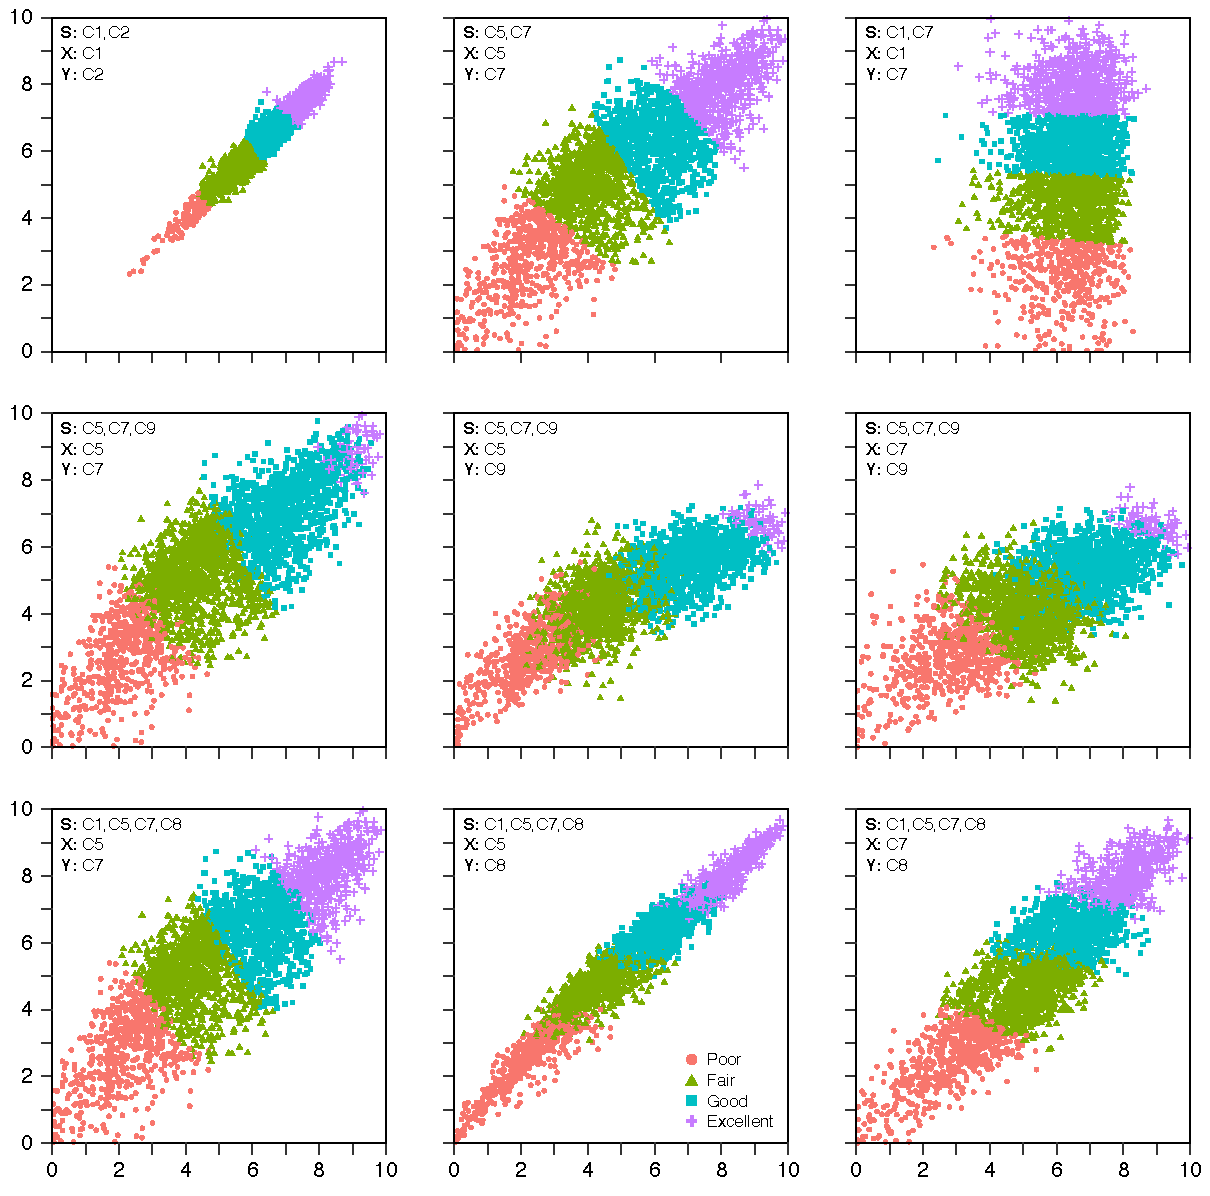
\includegraphics[width=\textwidth]{figures/pdf/figure-05}
	\caption{A sample of the results from the multi-dimensional clustering analysis showing the clusters from a two-dimensional perspective into the relationships between different GOF metrics. In each case, the labels near the upper-left corner indicate the features considered in the subspace analysis, and the features associated to the horizontal ($x$) and vertical ($y$) axes in the plot. The top, middle, and bottom rows correspond to 2-, 3-, and 4-feature subspace analyses. In each case, the poor, fair, good, and excellent clusters are indicated with circle, triangle, square, and cross symbols, respectively. The empty circles indicate the location of the artificial cannot-link stations we introduced as background knowledge to the clustering process. The color version of this figure is available only in the electronic edition.}
	\label{fig:clusters}
\end{figure*}

Figure \ref{fig:boxed-clusters} shows the statistical distribution (box-plots) of the samples once the dataset is partitioned into the four GOF validation classes. This is similar to Fig.~\ref{fig:data-box-plot}, but after the clustering process is completed. Separately, we prepared similar plots to look at the influence of the velocity models and components of motions on the results of the clustering process and, as observed before, they had no significant differences with the aggregate of all the samples in the dataset. \change{Figure 6 is particularly important because it highlights the outcome of the clustering process and provides a preview into the decision tree analysis results. Notice that metrics C5 through C8 consistently fall within the poor, fair, good, and excellent classification and that metrics C3 and C4 also show a progressive variation in sync with the validation classes. This means that these metrics are likely the best predictors for the outcome of the validation process, as we will see upon performing the decision tree analysis. On the other hand, metrics C1 and C2, and C9 through C11 are almost invariant, therefore less or not decisive in the validation process. C11, in particular, shows a broader (larger boxes) distribution, which indicates that it is less effective in predicting the final validation class.}

\begin{figure*}
	\centering
	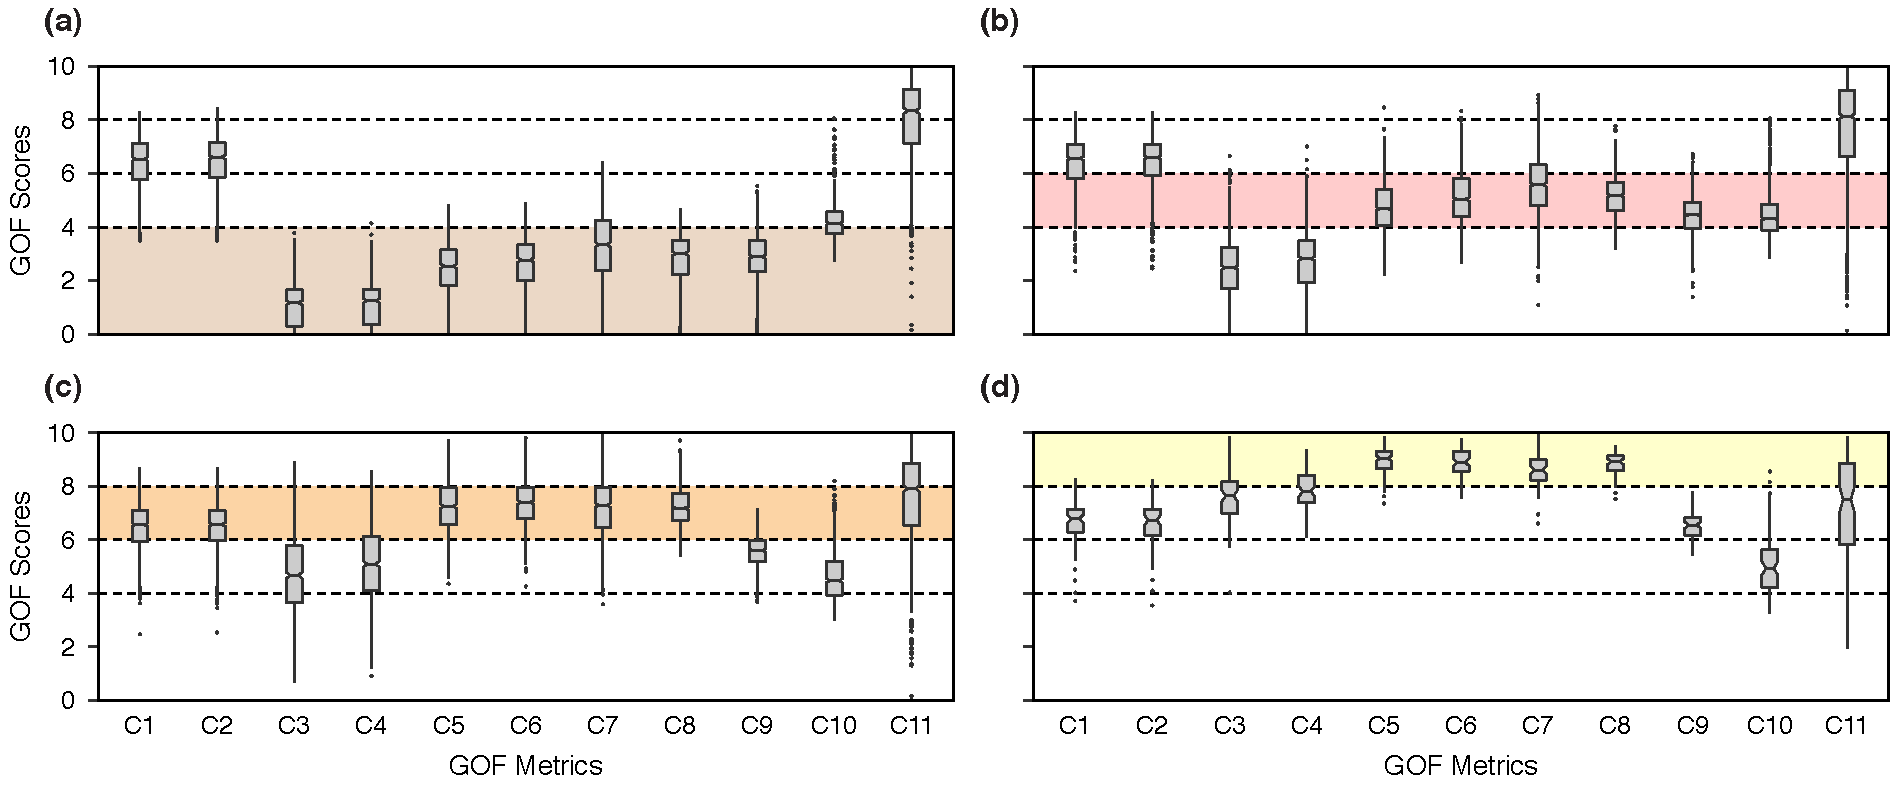
\includegraphics[width=\textwidth]{figures/pdf/figure-06}
	\caption{Statistical distribution of the dataset as partitioned into the four validation categories (poor, fair, good, excellent) after the clustering analysis. The distributions are shown in the form of box-plots for each metric (C1 through C11). In each case, \change{the medians are indicated by a notch in the boxes of the central quartiles, and the vertical} lines represent the interquartile range, with outliers shown as scattered dots. \change{The dashed lines and background shadows represent the boundaries of the poor, fair, good, and excellent categories as defined by \citet{Anderson_2004_Proc}.} The color version of this figure is available only in the electronic edition.}
	\label{fig:boxed-clusters}
\end{figure*}

In total, the clustering process results in 816, 1253, 879 and 76 data samples for the poor, fair, good and excellent classes, respectively. These groups are shown in Fig.~\ref{fig:count-classes}. As it can be seen in this figure, the number of samples in the excellent class is significantly less than those in the poor, fair, and good classes. Therefore, before moving on with the decision tree analysis, it is necessary to resample the subset of the excellent class\change{, for which we use the oversampling approach described in the previous section. Oversampling is nothing else but a replication of data samples. This process is done randomly, i.e., through a random selection of data samples from the original set to be duplicated until one increases the number of total samples in the oversampled set to a desired target number. In the case of the excellent class, we applied oversampling until reaching a total of 760 samples, as indicated with the dashed line in Fig.~\ref{fig:count-classes}. Since the original size was 76 samples, that means we applied an oversampling ratio of 10$\times$. According to \citet{Weiss_2003_JAIR}, an oversample rate of 10$\times$ is considered to be acceptable in this type of data processing.} (Arguably, we could have as well undersampled the fair class, but we deemed that unnecessary. Instead, we used a \change{heavy} pruning process to prevent overfitting.) Once this process was completed we went on with the decision tree analysis.

% We used the oversampling approach described in the previous section. We replicated data from the excellent class 
% \myrevision{through random selection of data from that class until elevating the number of samples in this class to 760 as indicated in Fig.~\ref{fig:count-classes} with the dashed line. This oversampling is considered as a $\times$10 factor.} 
% \myremove{randomly by a $\times$10 factor until elevating the number of samples in this class to 760 as indicated in Fig.~\ref{fig:count-classes} with the dashed line.} 
% By common standards, an oversample rate of $\times$10 is considered acceptable \citep{Weiss_2003_JAIR}. 

\begin{figure}[t]
	\centering
	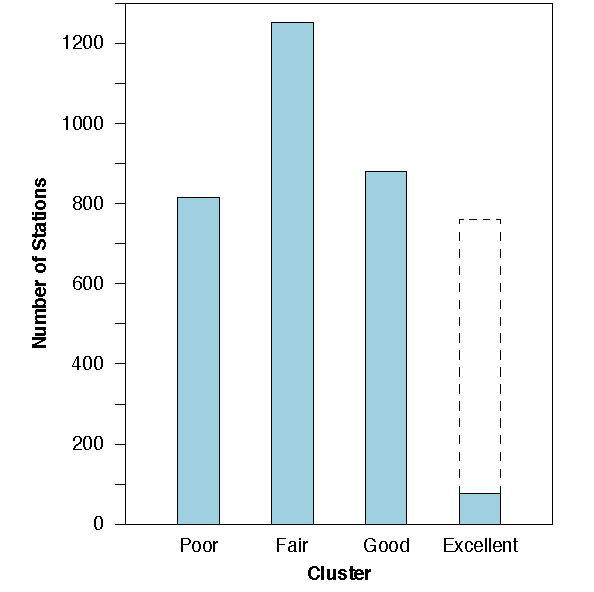
\includegraphics[width=0.45\textwidth]{figures/pdf/figure-07}
	\caption{Number of data samples in each class (poor, fair, good, excellent) after conducting a multi-dimensional constrained \kmeans{} clustering process using subspace analysis for 2, 3, and 4 features (GOF metrics). The dashed-line bar indicates the number of samples in the excellent class after oversampling. The color version of this figure is available only in the electronic edition.}
	\label{fig:count-classes}
\end{figure}

In total we generated 20,000 trees using the C5.0 algorithm for all possible combinations of the parameters CF and $S_{\min}$, where CF was chosen to vary between 0 and 1 at intervals of size 0.01, and $S_{\min}$ was chosen to vary between 1 and 200 at unitary intervals. Despite our choice for small intervals, the algorithm often reached recurrent tree structures for different CF and $S_{\min}$ values. Therefore, in reality, from the 20,000 combinations for which we ran the algorithm, only 66 unique trees were found. 

\begin{figure*}[t]
	\centering
	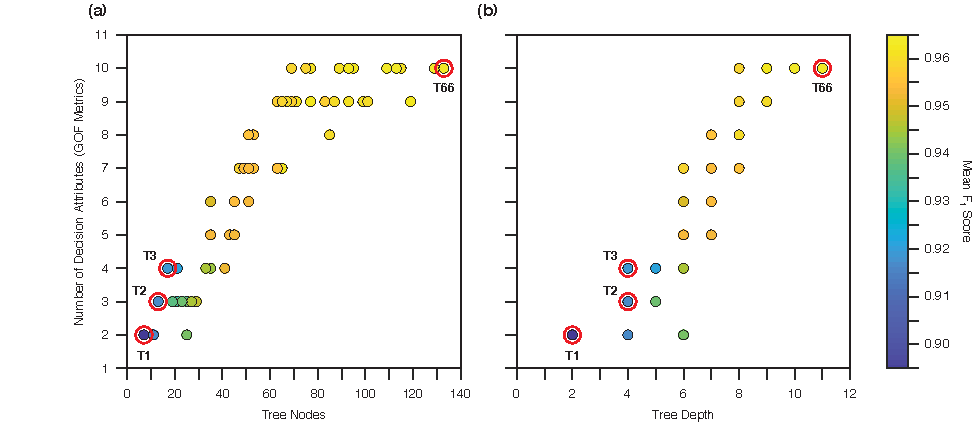
\includegraphics[width=\textwidth]{figures/pdf/figure-08}
	\caption{Accuracy of tree predictions in terms of the factor ($F_1$) from equation \ref{eq:f} as indicated by colored dots distributed with respect to the number of attributes (GOF metrics) as a function of: \textbf{(a)} the number of nodes, and \textbf{(b)} the depth of the trees. The rings around some of the dots indicate select trees used as reference in the text, other figures and tables. The color version of this figure is available only in the electronic edition.}
	\label{fig:nodes-depth}
\end{figure*}

\begin{table}[t]
	\centering
	\caption{Confusion matrix results for decision tree T1}
	\label{tab:t1:confusion}
	\small
	\begin{tabular}{cccccc}
		& 		& \multicolumn{4}{c}{Prediction}\\ 
		\cline{3-6}
		&   	& P  	& F     & G  	& E 	\\
		\cline{2-6}
		\parbox[t]{2mm}{\multirow{4}{*}{\rotatebox[origin=c]{90}{Actual}}}  
		& P 	& 242 	& 11 	& 0     & 0    	\\
		& F 	& 13 	& 313   & 16    & 0    	\\
		& G 	& 0 	& 42    & 207   & 15   	\\
		& E 	& 0 	& 0     & 23    & 231	\\ 
		\cline{2-6}
	\end{tabular}
\end{table}

\begin{table}[t]
	\centering
	\caption{Confusion matrix results for decision tree T3}
	\label{tab:t3:confusion}
	\small
	\begin{tabular}{cccccc}
		& 		& \multicolumn{4}{c}{Prediction}\\ 
		\cline{3-6}
		&   	& P  	& F     & G  	& E 	\\
		\cline{2-6}
		\parbox[t]{2mm}{\multirow{4}{*}{\rotatebox[origin=c]{90}{Actual}}}  
		& P 	& 248 	& 14 	& 0     & 0    	\\
		& F 	& 7 	& 343   & 18    & 0    	\\
		& G 	& 0 	& 9 	& 221   & 33   	\\
		& E 	& 0 	& 0     & 7    	& 213	\\ 
		\cline{2-6}
	\end{tabular}
\end{table}

For each one of these unique trees, we computed the effectiveness factor $F_1$ from equation (\ref{eq:f}), and extracted the total number of nodes in the trees and their depth. Figure \ref{fig:nodes-depth} shows the results of $F_1$ for all the trees and its distribution in terms of the number of \change{decision} attributes \change{or GOF metrics} used in the trees as a function of the number of nodes and the depth of each tree. Recall that we are interested in finding a sequence of decisions (represented by disjunctive decision nodes in a tree) that can lead to good GOF predictions (i.e, high values of $F_1$) using a reduced number of attributes (GOF metrics). In general, all the trees obtained with the C5.0 algorithm are good in terms of the effectiveness factor ($F_1$ values close to 1). Then our choice comes down to using a reduced number of metrics. Having several trees with 2, 3, and 4 metrics (as opposed to 11), the following factor in the decision is choosing trees with algorithms using a small number of steps to reach the prediction. This is given by a combination between the depth of the tree and the number of nodes in the tree (i.e., trees with low complexity).

Based on these criteria, we selected three candidate trees: T1, T2, and T3. These trees are shown in Fig.~\ref{fig:trees}. T1 is the simplest of the three, and T2 and T3 share some of their topology on the right-hand side. T3 is the most complex of them. More complex trees tend to be deeper, have more nodes, and employ more attributes. \myrevision{complexity of trees is controlled by pruning process.} This leads to higher $F_1$ values, but they may not necessarily be more practical. In total T1, T2, and T3 use 2, 3 and 4 attributes respectively. All coincide in the use of the total energy (C4) and response spectra (C8) as key metrics. T2 adds peak acceleration (C5), and T3 adds peak velocity \change{(C6)} to the previous metrics.

\begin{figure*}
	\centering
	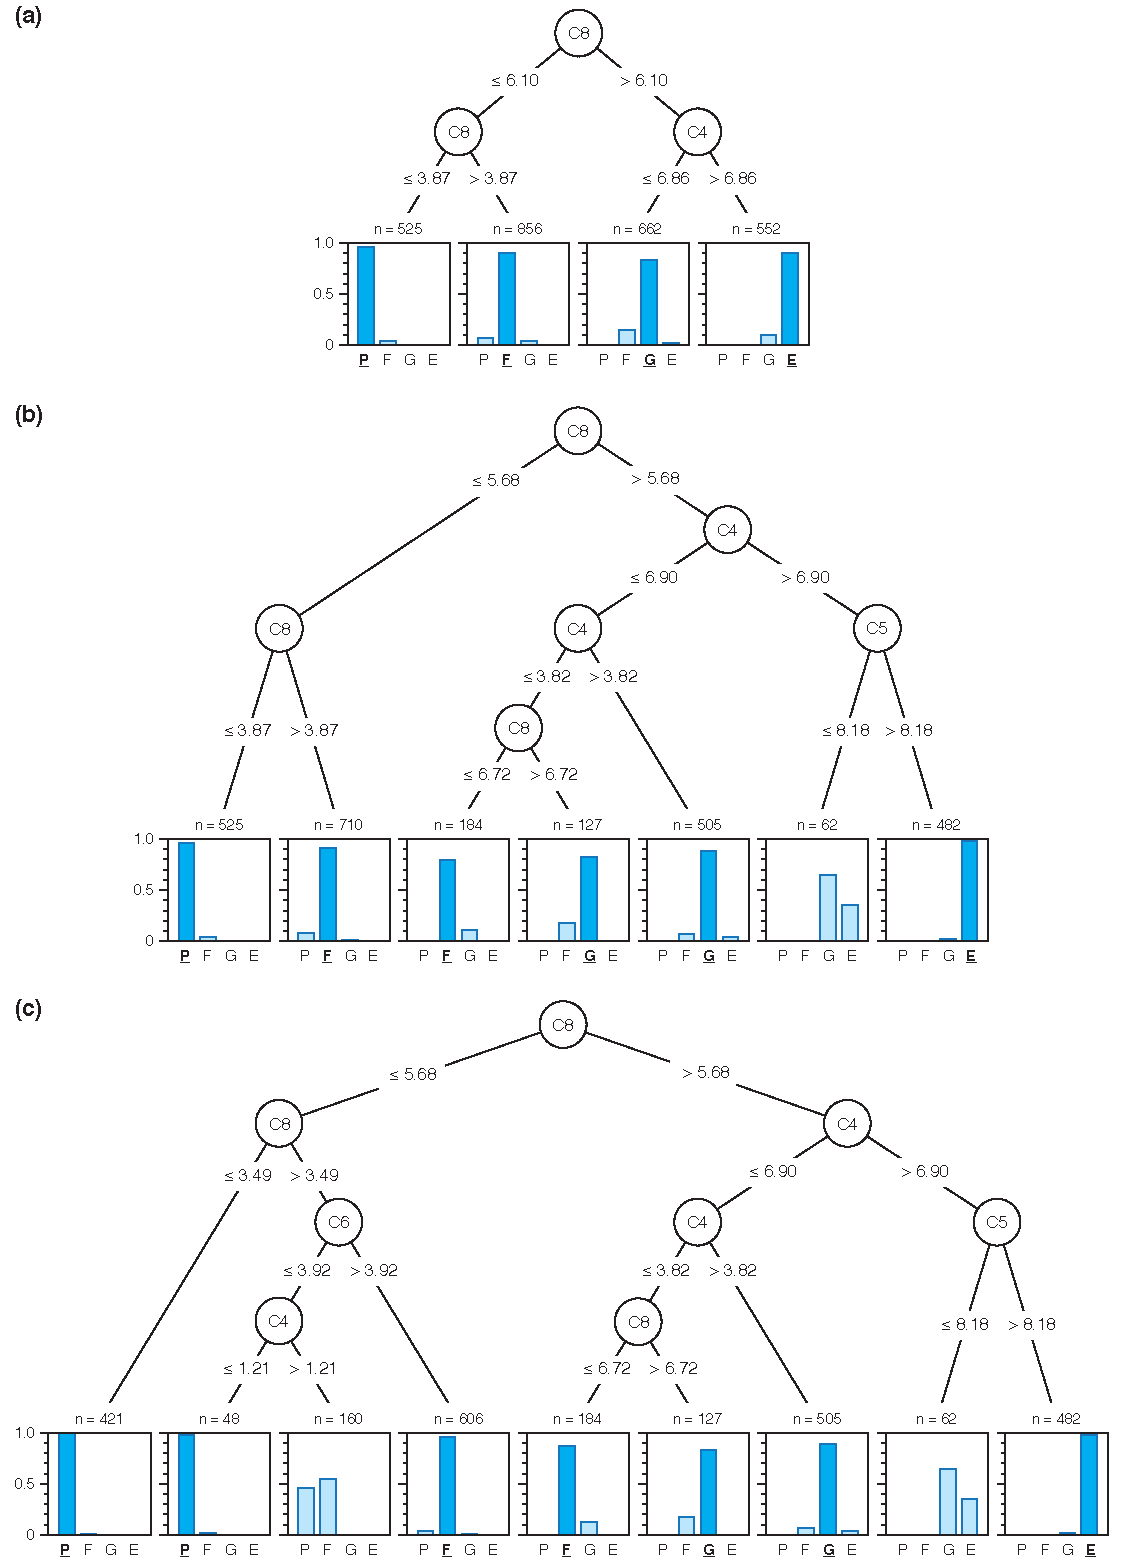
\includegraphics[width=0.86\textwidth]{figures/pdf/figure-09}
	\caption{Selected trees \textbf{(a)} T1, \textbf{(b)} T2, and \textbf{(c)} T3. In each case the decision nodes of the trees contain the code corresponding to the metric (see Table \ref{tab:metrics}) used and the branches beneath each node show the limit value to be used to select the next level in the tree. At the bottom, normalized histograms are shown to indicate the distribution of the samples at each leaf-node according to the validation classes with codes P, F, G, and E for poor, fair, good, and excellent, respectively. At the top of each histogram is the total count of samples at the corresponding leaf node. The histograms highlight the dominant validation class. The color version of this figure is available only in the electronic edition.}
	\label{fig:trees}
\end{figure*}

\begin{table}[t]
	\centering
	\caption{T1 precision, recall, and $F_1$ values per class}
	\label{tab:t1:f1}
	\small
	\begin{tabular}{lccc}
	Class   & $P$	& $R$  	& $F_1$ \\ 
	\hline
	P 		& 0.96 	& 0.95 	& 0.95 	\\
	F 		& 0.92 	& 0.86 	& 0.88 	\\
	G 		& 0.78 	& 0.84 	& 0.81 	\\
	E 		& 0.91 	& 0.94 	& 0.92 	\\
	\hline
	Mean 	&		&		& 0.90	\\
	\end{tabular}
\end{table}

\begin{table}[t]
	\centering
	\caption{T3 precision, recall, and $F_1$ values per class}
	\label{tab:t3:f1}
	\small
	\begin{tabular}{lccc}
	Class   & $P$	& $R$  	& $F_1$ \\ 
	\hline
	P 		& 0.95 	& 0.97 	& 0.95 	\\
	F 		& 0.93 	& 0.93 	& 0.93 	\\
	G 		& 0.84 	& 0.89 	& 0.86 	\\
	E 		& 0.96 	& 0.86 	& 0.91 	\\
	\hline
	Mean 	&		&		& 0.91	\\
	\end{tabular}
\end{table}

At the bottom of each tree in Fig.~\ref{fig:trees} are the histograms of the data that land on each leaf node. (Note that the count of samples here is done based on the training dataset.) The decision tree assigns the final validation category based on the dominant class in each leaf. As such, the samples in the second leaf-node from the right in T3 are categorized as good despite a significant portion of them being excellent. This is a natural trade-off embedded in the use of \myrevision{pruned} decision trees which actually results in more effective trees. 

The actual effectiveness (i.e., the average $F_1$ values shown in Fig.~\ref{fig:nodes-depth}), however, is measured based on the testing dataset. Recall that $F_1$ depends on the number of true predictions and false predictions measured by the confusion matrix and the precision and recall factors. Tables \ref{tab:t1:confusion} and \ref{tab:t3:confusion} show the confusion matrices for T1 and T3, respectively; and Tables \ref{tab:t1:f1} and \ref{tab:t3:f1} show the corresponding results for $P$, $R$, and $F_1$. As it can be seen in the Tables \ref{tab:t1:confusion} and \ref{tab:t3:confusion}, both trees lead to strong diagonal confusion matrices, meaning that the classification into poor, fair, good and excellent is well defined. The differences between both matrices are actually minor and small with respect to their diagonal values, and the $F_1$ values in Tables \ref{tab:t1:f1} and \ref{tab:t3:f1} are all near to or above 0.9. The values obtained for tree T2 are consistent with this.

Another aspect of interest is the level of participation of each metric in the analysis of data as GOF values are run through the decision nodes in the trees. The results of such level of participation are listed in Table \ref{tab:participation} for trees T1, T2, T3, and T66. (The tree T66 is the most complex of them all as inferred from the number of metrics involved and the number of nodes and levels as seen in Fig.~\ref{fig:nodes-depth}.) The percentages in this table represent the amount of data that is seen by a decision node associated by any particular metric. The nodes are not unique and metrics are often used in different nodes in a given tree, thus these percentage are cumulative for each individual metric. A percentage of 100 means a given metric has the opportunity to see all data samples through a single nodes or multiple ones. A low percentage means only a few data samples are evaluated by that metric, and a null percentage means the metric plays no role in the decision tree (it is not present in any node).

Notice that in all trees \myrevision{,using all metrics,} the metrics C4 (total energy) and C8 (response spectra) are consistently the most relevant ones in the decision algorithms. They are followed by C5 (peak acceleration) and C6 (peak velocity). On the other end, notice that C11 (strong phase duration) plays no role whatsoever in any of the trees, and that C1 (Arias integral), C2 (energy integral), and C3 (Arias intensity) have only small to marginal participations. The remaining metrics---C7 (peak displacement), C9 (Fourier spectrum), and C10 (Cross correlation)---have a somewhat significant participation, but only in the more complex trees.

\myrevision{It is obvious that C8(response spectra) and C5(peak acceleration) are the most important metrics in developing the prediction models. Therefore, in order to understand other parameters importance we developed two sets of trees according to complexity of the original trees (the structure of generated trees are not presented here), while once dropping C8 (response spectra) and once dropping C8 (response spectra) and C5(peak acceleration) from the prediction attributes. According to Table \ref{tab:participation}, these trees also emphasize the importance of C4 and C6. However, in the absence of C5(peak acceleration) and C8 (response spectra),  C3 (Arias intensity) and C9 (Fourier spectrum) become more effective in developing prediction models. Also C11(strong phase duration) becomes somewhat important in the most complicated tree.}

A low participation does not necessarily mean that a given metric is not important. Arguably, the strong phase duration is highly regarded as an important parameter for strong motion records in engineering. What the results we present here mean \change{is that, in the context of this particular set of 11 metrics, in order to classify whether a simulation result is poor, fair, good, or excellent, other metrics such as energy (C8) are much more influential in the final result than the duration (C11). This, of course, is done under the assumption that one seeks to narrow the selection of metrics without loss of insight about the outcome of the validation process when compared to the outcome obtained with the whole suite of the eleven metrics used here.}

% Original:
% A low participation does not necessarily mean that a given metric is not important. Arguably, the strong phase duration is highly regarded as an important parameter for strong motion records in engineering. What the results we present here mean, in the context of GOF validation, is that in order to classify whether a simulation result is poor, fair, good, or excellent, other metrics such as energy (C8) are much more decisive in reaching an accurate conclusion about validation quality than the duration (C11).

% Naeem suggestion:
% A low participation does not necessarily mean that a given metric is not important. Arguably, the strong phase duration is highly regarded as an important parameter for strong motion records in engineering. What the results we present here mean, in the context of GOF validation for engineering applications, is that in order to classify whether a simulation result is poor, fair, good, or excellent, other metrics such as energy (C8) are much more decisive in narrowing eleven validation metrics into fewer numbers in order to get the same categorization as all eleven metrics than the duration (C11).

In the end, the final selection of a preferred tree comes down to reducing complexity in the analysis without compromising the interpretation of results. We favor tree T1 because it is based only in three decision steps, and two GOF metrics: C4 (total energy), and C8 (response spectra).


\begin{table}[t]
	\centering
	\caption{Metrics data analysis participation (in percent) for select trees }
	\label{tab:participation}
	\small
	\begin{tabular}{lrrrr}
	Metric 	& T1 	& T2	& T3 	& T66 	\\ 
	\hline
	C1 		& --	& --	& -- 	& 1.5	\\
	C2 		& -- 	& --	& -- 	& 0.5	\\
	C3 		& -- 	& -- 	& -- 	& 9.6	\\
	\rowcolor{light-light-gray}
	C4 		& 46.8	& 52.4	& 60.2	& 100.0	\\
	\rowcolor{light-light-gray}
	C5 		& -- 	& 21.5	& 21.5	& 72.2	\\
	\rowcolor{light-light-gray}
	C6 		& -- 	& -- 	& 37.0	& 56.3	\\
	C7 		& -- 	& -- 	& -- 	& 19.4	\\
	\rowcolor{light-light-gray}
	C8 		& 100.0	& 100.0	& 100.0	& 100.0	\\
	C9 		& -- 	& -- 	& --	& 23.8	\\
	C10		& -- 	& -- 	& -- 	& 22.2	\\
	C11		& -- 	& -- 	& -- 	& -- 	\\
	\hline
	\end{tabular}
\end{table}





\begin{table*}[t]
	\centering
	\caption{Data analysis participation (in percent) for select trees after removing certain metrics}
	\label{tab:participation-extra}
	\small
	\begin{tabular}{llrrrrcrrrr}
	& & \multicolumn{4}{c}{Without C8}		& 	& \multicolumn{4}{c}{Without C5 and C8}\\
	\cline{3-6} \cline{8-11}
	\multicolumn{2}{l}{Metric} 	& T1 	& T2	& T3 	& T66 	&	& T1 	& T2	& T3 	& T66 	\\ 
	\hline
	C1 		& Arias Integral	& --	& --	& -- 	& --	&	& --	& --	& -- 	& --	\\
	C2 		& Energy Integral	& --	& --	& -- 	& 2.27	&	& --	& --	& -- 	& --	\\
	C3 		& Arias Intensity	& --	& --	& -- 	& 53.2	&	& --	& 60.4	& 61.2	& 99.1	\\
	C4 		& Total Energy		& 44.3	& 81.8	& 81.8	& 83.2	&	& 47.44	& 48.7	& 80.5	& 54.6	\\
	C5 		& Peak Acc.			& 100.0	& 100.0	& 100.0	& 100.0	&	& --	& --	& -- 	& --	\\
	C6 		& Peak Vel.			& 58.6	& 63.5	& 62.8	& 82.4	&	& 100.0	& 100.0	& 100.0	& 100.0	\\
	C7 		& Peak Disp.		& --	& --	& -- 	& 32.4	&	& --	& --	& -- 	& 43.2	\\
	C8 		& Response Spec.	& --	& --	& -- 	& --	&	& --	& --	& -- 	& --	\\
	C9 		& Fourier Spec.		& --	& --	& -- 	& 48.6	&	& --	& --	& -- 	& 72.2	\\
	C10		& Cross Corr.		& --	& --	& -- 	& 24.9	&	& --	& --	& -- 	& 20.5	\\
	C11		& Strg.~Phase Dur.	& --	& --	& -- 	& --	&	& --	& --	& -- 	& 8.09	\\
	\hline
	\end{tabular}
\end{table*}






% \section{Verification Test}
\section{\change{Testing}}

We now \change{test} tree T1 on the original simulation results from \citet{Taborda_2014_BSSA}, for different velocity models and components of motion. In this case we no longer aggregate all data from the simulation but now look at individual simulations done with different velocity models, and the three components of motion separately, as it would normally be done during any ground motion simulation validation. The results obtained with the T1 validation algorithm are shown in Fig.~\ref{fig:res-gof-maps}. \change{In an ideal case, we would expect these results to closely resemble those obtained by \citet{Taborda_2014_BSSA}, if grouped only into four categories. Relying only on the two metrics C4 and C8 using T1 is, however, not exactly the same. In addition, a}
% 
% These results are in essence very similar to those obtained by \citet{Taborda_2014_BSSA}, though using the T1 algorithm, we now rely only on the two metrics C4 and C8.
% 
% A relative 
drawback from the T1 algorithm is that because its outcome are GOF validation classes (poor, fair, good, excellent) as opposed to GOF validation scores (with values from 0 to 10), once one obtains the results for the validation process for different components of motion (as shown in the rows of Fig.~\ref{fig:res-gof-maps}), there is no natural way of taking averages as one would do for scores in a numerical scale \change{\citep[i.e., as typically done when using][]{Anderson_2004_Proc}}. Therefore, in order to combine results from the three components into a single validation classification for each station, we define the following rules:

\begin{itemize}
	\setlength\itemsep{0ex}
	\item If the three components share the same validation class, then that class is assigned as the combination result.
	\item If two components share the same validation class, but one differs, then the class shared by the former two is assigned as the combination result, thus favoring the majority.
	\item If all three components have different validation classes, then the final combination result is set as the lower class of the three, penalizing the lack of conclusive results.
\end{itemize}

We call the result of applying these rules a tree T1 combination. Applying them to the validation results shown in Fig.~\ref{fig:res-gof-maps} for the case of the simulation done using the model CVM-S is shown in Fig.~\ref{fig:avg-gof-maps}, which compares the outcome with the result of the average scores obtained using the traditional \citet{Anderson_2004_Proc}-type GOF method. This figure exemplifies the \change{differences or similarities} between the numeric GOF validation-scores scale and the proposed T1 GOF validation classes. 
% At the same time, it highlights the similarities between the outcomes.

\begin{figure*}%[th!]
	\centering
	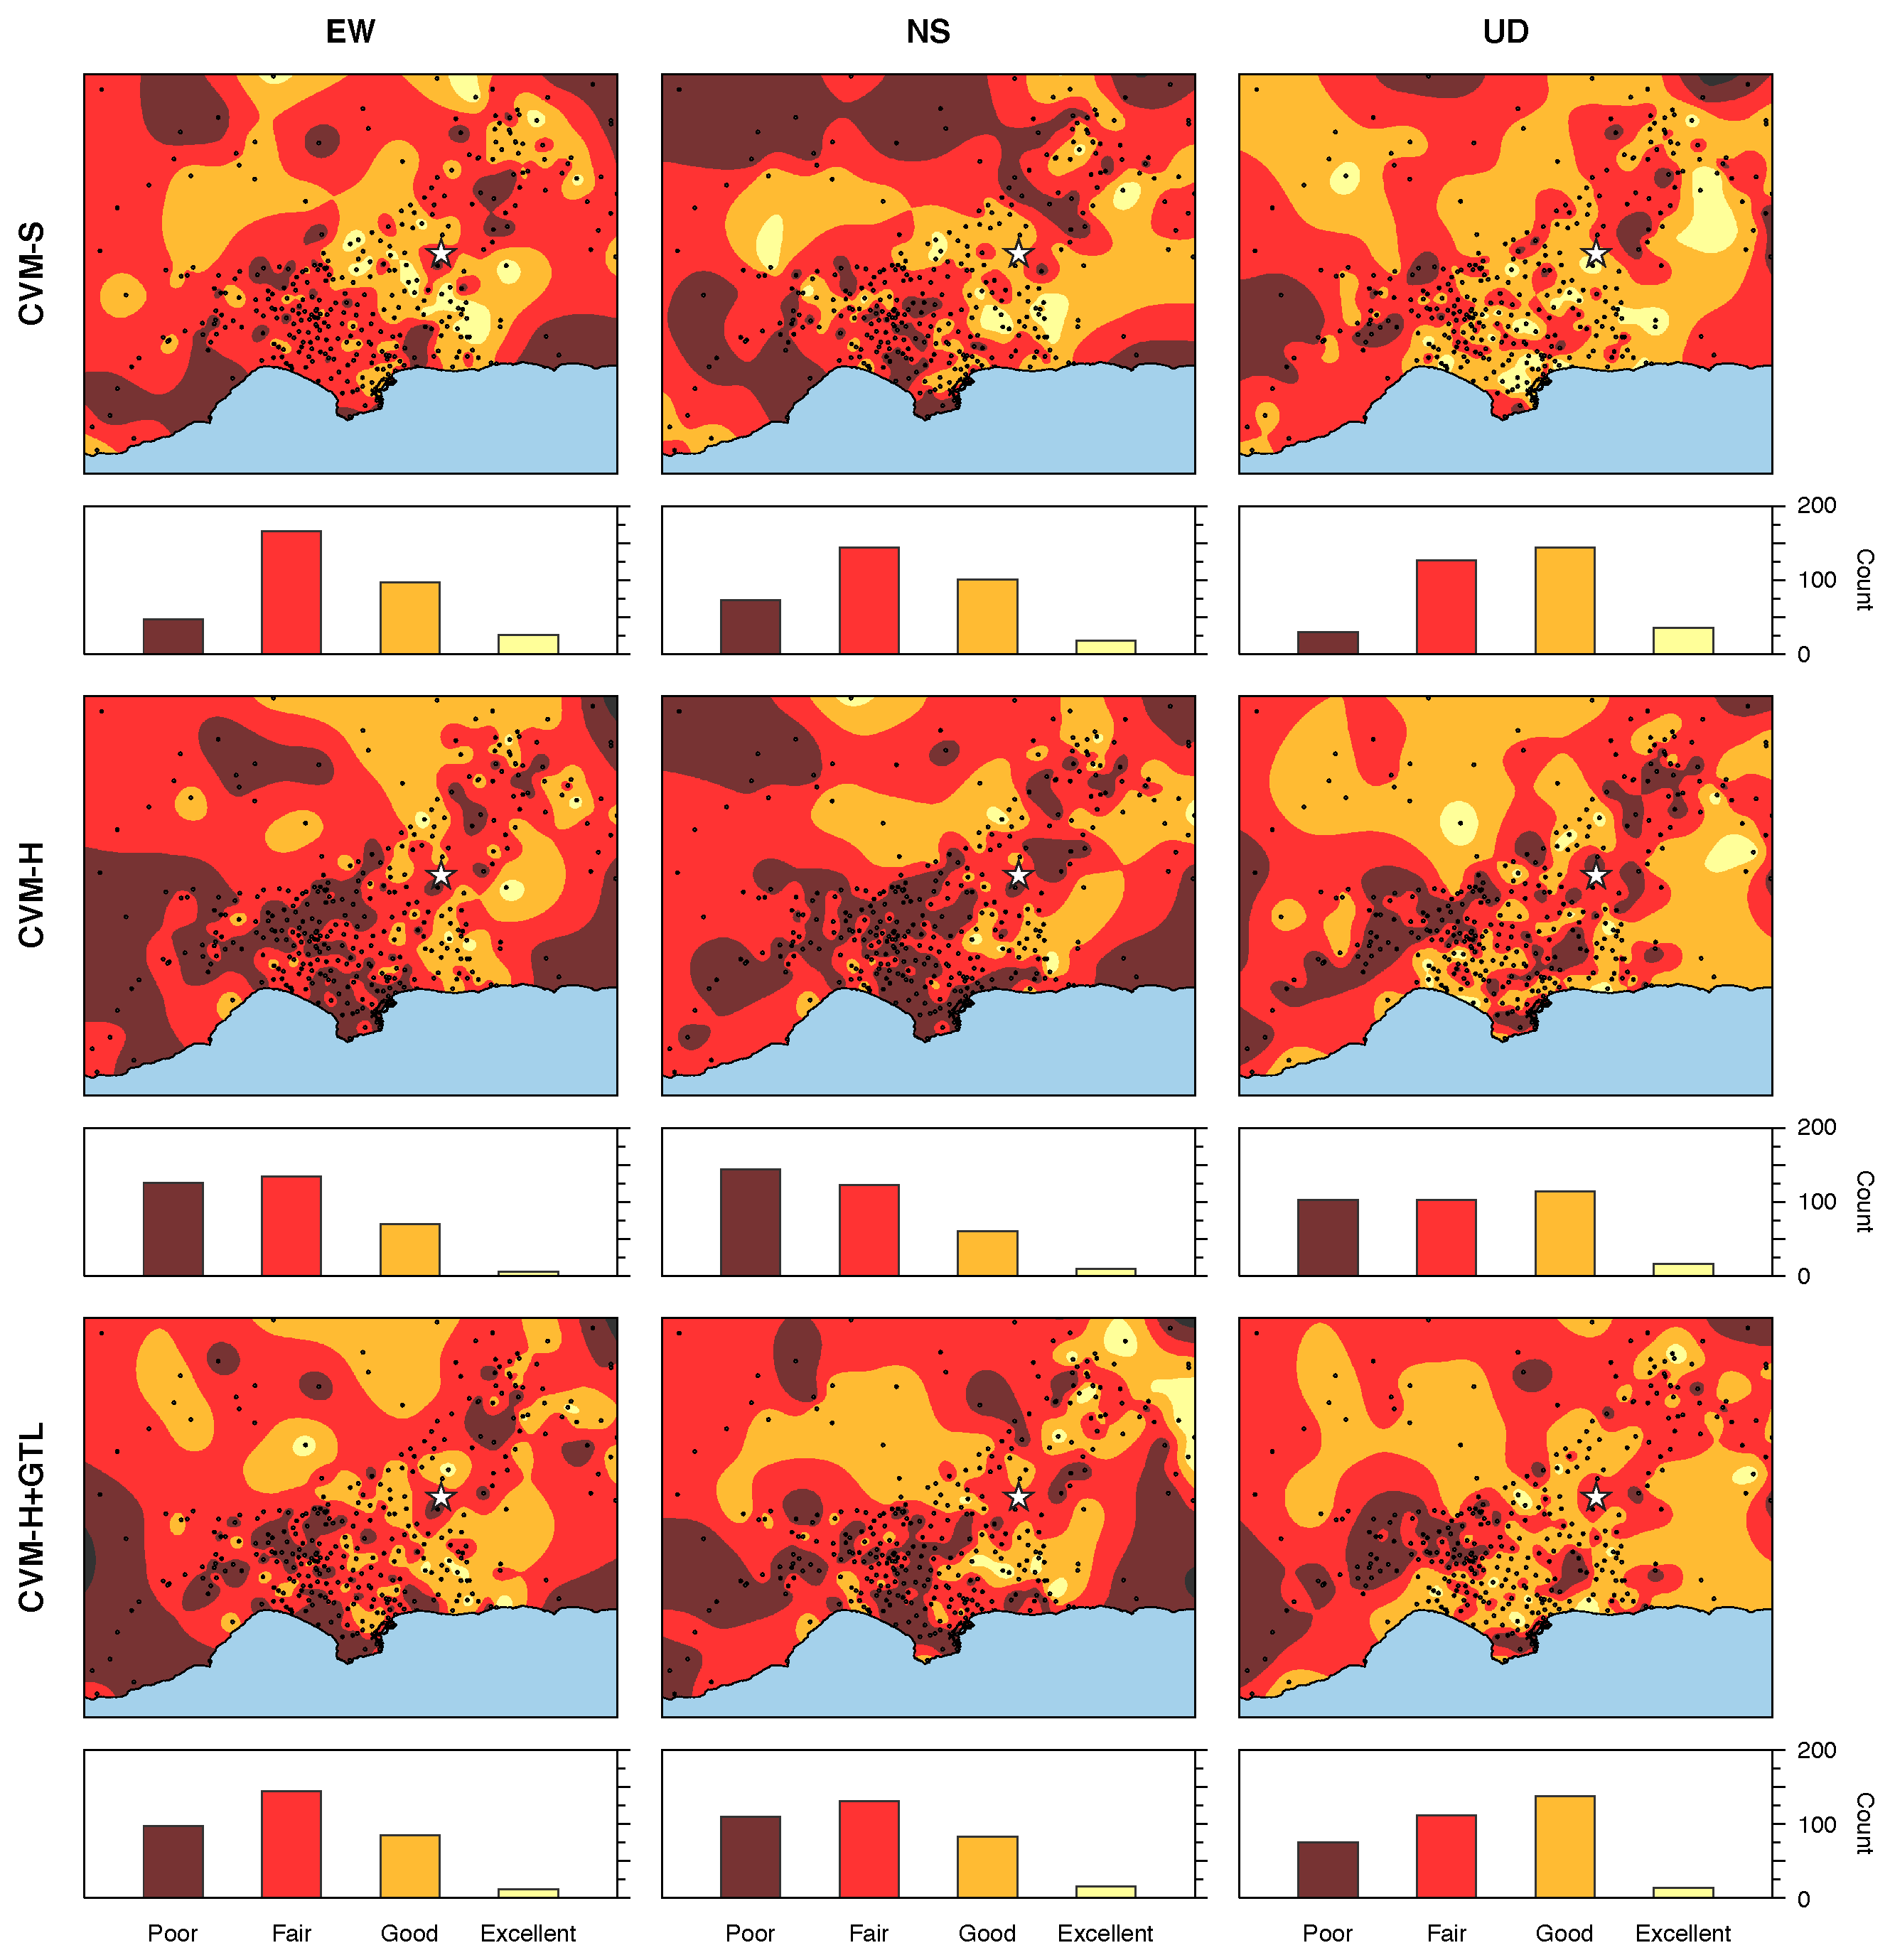
\includegraphics[width=\textwidth]{figures/pdf/figure-10}
	\caption{Results obtained using the validation algorithm of the selected decision tree T1 on the 2008 Chino Hills earthquake simulation results reported by \citet{Taborda_2014_BSSA}. Here, the validation process is carried out separately for each component of motion (EW, NS, UD), for three different simulations corresponding to simulations done using the southern California velocity models: CVM-S, CVM-H, CVM-H+GTL. The contours maps are drawn for illustration purposes only based on the spatial distribution of the GOF validation class assigned to each station. The bottom histograms show the count of stations in each validation class. Stations are indicated with dots, and the epicenter with a Star. The color version of this figure is available only in the electronic edition.}
	\label{fig:res-gof-maps}
\end{figure*}

In our view, the T1 results are simpler to assimilate and equally informative. Looking at both plots in Fig.~\ref{fig:avg-gof-maps} it is possible to argue they lead to \change{similar conclusions in respect to the overall validation of the simulation, and in respect to some particular areas and specific locations. Nonetheless, it must be said that we do not expect to see a 1-to-1 relationship. That is the scope of a future work, whereas here our focus was on identifying the relevance of the different metrics. This is important because the original approach proposed by \citet{Anderson_2004_Proc} favors a uniform weighing of metrics, and the results shown here indicate this may not be the preferred strategy.}

% conclusions and present a similar picture of the validation of the simulation, not only globally but at specific locations, with only minor differences---especially if one is to consider the assumed equivalence between scores and classes (0--4: poor; 4--6: fair; 6--8:good; 8--10: excellent). \myrevision{However, we do not expect to see the same results in both figures. \citet{Taborda_2014_BSSA} results is developed based on assigning uniform weight on all metrics, however, this study research question is addressing the importance of different metrics and implying that assigning uniform weights might not provide accurate results.}

\begin{figure*}[th!]
	\centering
	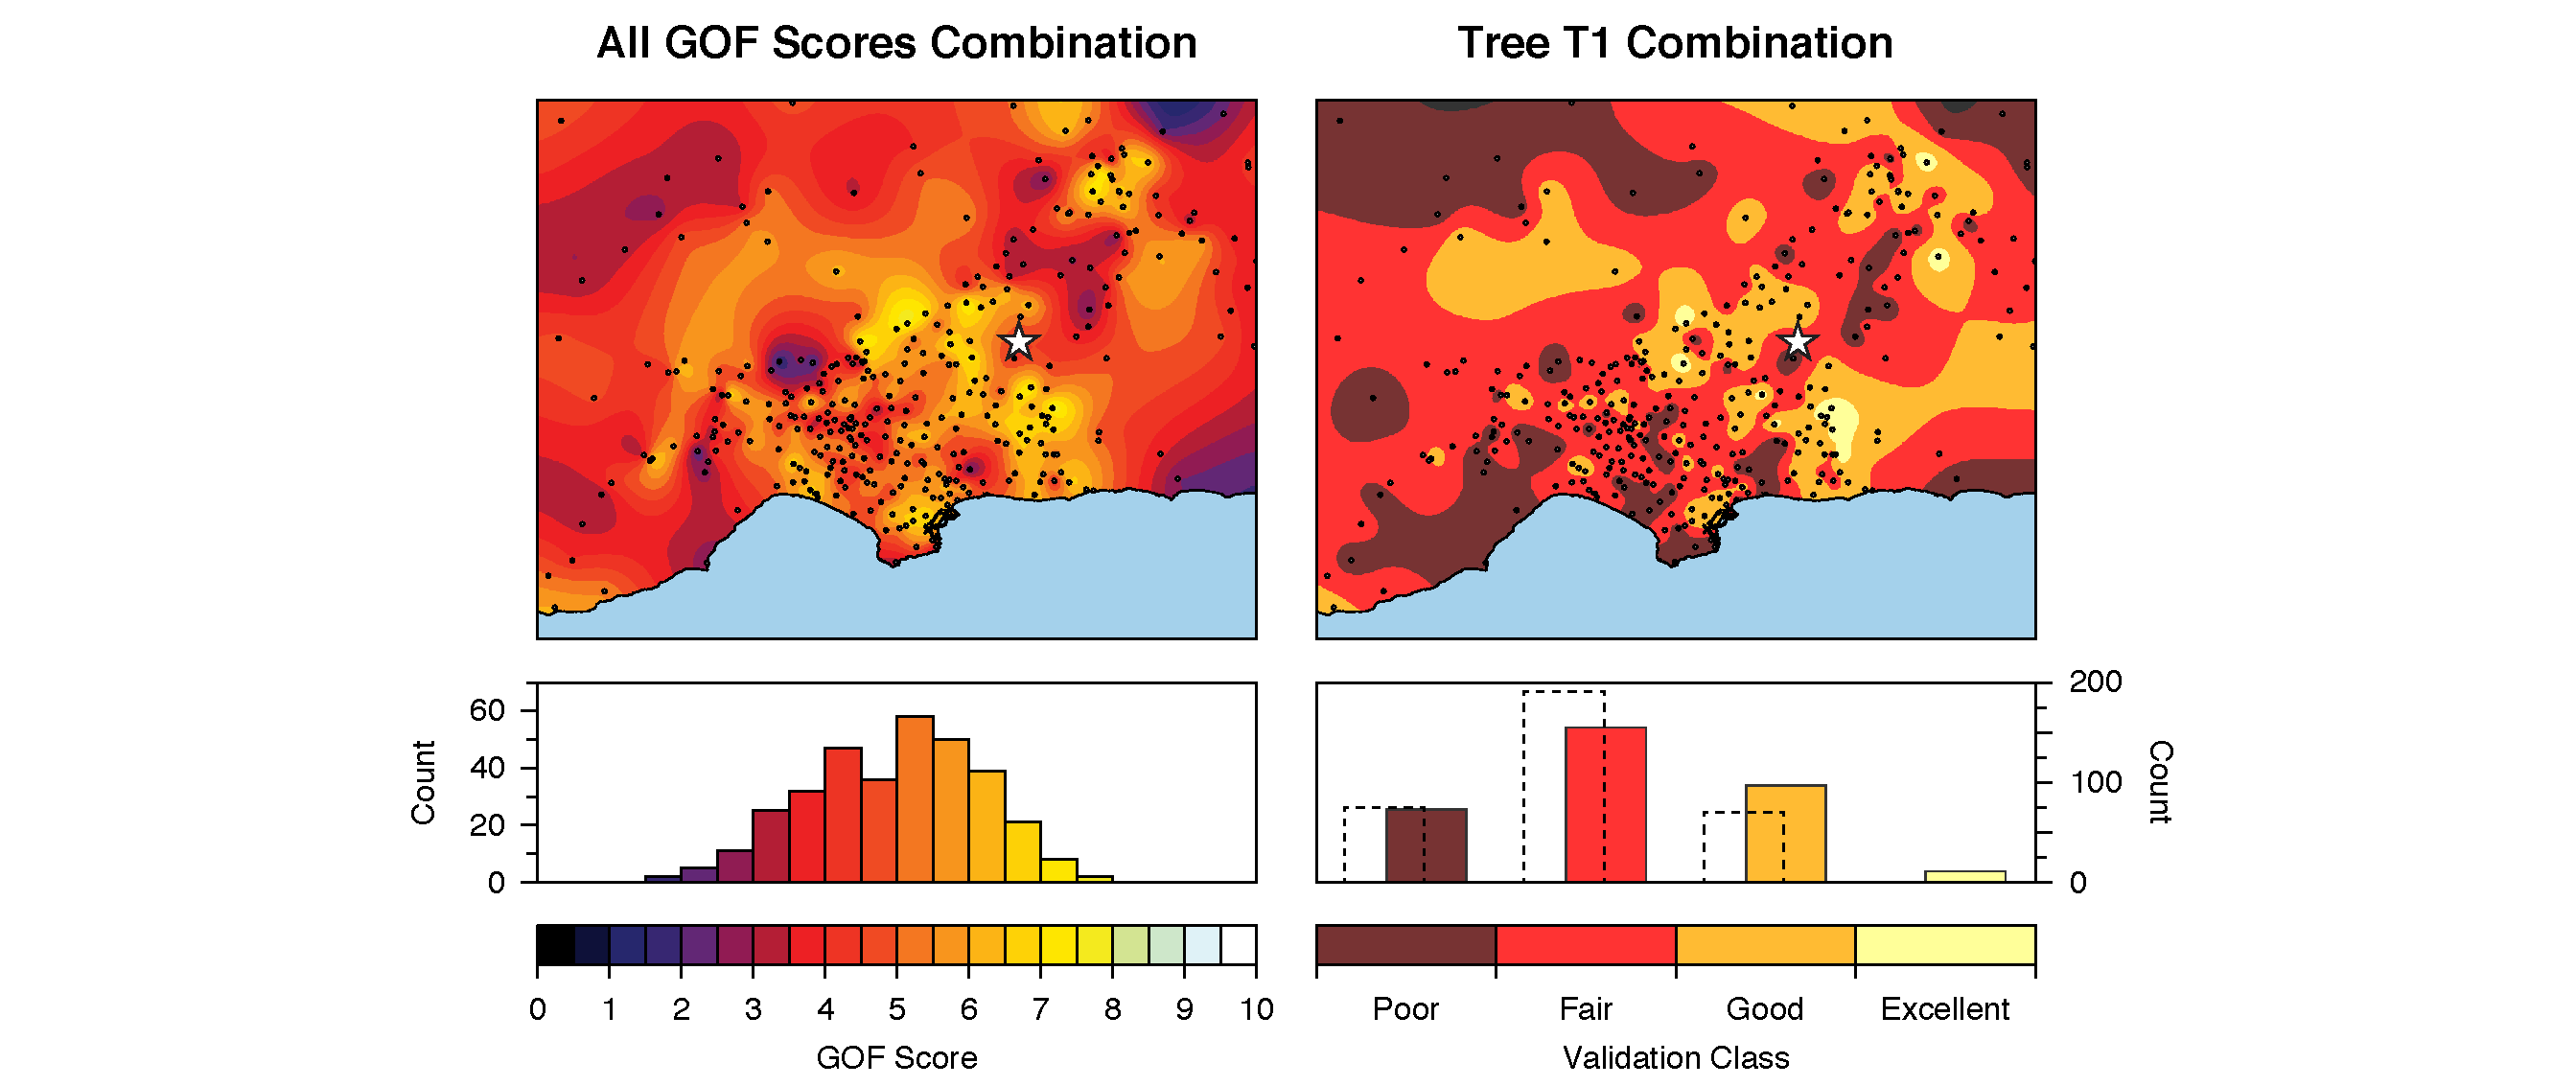
\includegraphics[width=\textwidth]{figures/pdf/figure-11}
	\caption{Comparison of GOF validation scores obtained using an 11-metric \citet{Anderson_2004_Proc}-type GOF scoring (left) and the T1 combination GOF validation classification (right). The top plots show maps with a distribution of the scores or classes outcome at each station. The contours are drawn for illustration purposes only. The bottom plots show histograms with the count of stations for each GOF score interval or validation class.}
	\label{fig:avg-gof-maps}
\end{figure*}

% \myrevision{It is worth mentioning that, in this study, we presented an integration of scientists knowledge and field data using machine learning algorithms to develop an acceptable and robust prediction model. This method can be used in any field where there are some field data as well as expertise knowledge about the data. Validation metrics are note limited to \citeauthor{Anderson_2004_Proc}'s metrics. Therefore, adding more metrics from different field can be used through the proposed method to develop prediction models. }








% 
\section{Discussion}

According to the results Response Spectra (C8) is the most important metric in classifying the stations. Data percentage in Table.~\ref{tab:attribute_usage_1} represent the amount of data that the attribute is used in classifying them.  After C8, Arias Intensity Value is the most effective metric. With $C8 \leq 4.07~ \& ~ 4.07 < C8 \leq 6.1$ and $6.1 < C8~ \&~ 6.87 \leq C4$ and $6.87 \leq C4 ~ \&  6.1 \leq C8$ one can classify the simulation as poor, fair, good, and excellent, respectively, with a high confidence.  In this case minimum F1-score occurs for Class 3 and maximum F1-score occurs for Class 1. Pruning process reduce the effect of oversampling in cluster 4. In the second model, which is more accurate from the first model for all metrics, other than Response Spectra and Total Energy, 3 other metrics including: Peak Velocity, Peak Acceleration, and Cross Correlation, also determines the classes.  Fig.~\ref{fig:C8dist} represents the variation of Response Spectra score in different distances for different velocity models and components. As one can see it is fairly well distributed in different score variation in respect to response. There is differences in median value in different components. The median value improves from CVMH+without GTL layer to CVMS. 

\begin{figure}
    \centering
    \includegraphics
       % [width=\columnwidth]
        [width=\textwidth]
        {figures/pdf/Figure_15.pdf}
    \caption{Variation of C8 (Response Spectra) score with distance. Velocity models are represented in different shapes and components in different colors.  }
    \label{fig:C8dist}
\end{figure}

Analysis of statistical significance for relevance of results to earthquake, velocity model, frequency band, magnitude, distance of stations, and components needs comprehensive study beyond clustering and classification. However, we illustrate the effects without making strong decision whether they affect the results or not. More comprehensive study is undergoing with \citet{Taborda_2016_GJI} dataset. \\
Finally, we represent the application of these models on classifying stations on a geographical representation. Fig.~\ref{fig:M1_dtree_gof} represent the application of the first decision tree algorithm on the simulation of Chino Hills earthquake. In order to keep consistency in color code, and be able to compare the results with other published results \citep[e.g.,][]{Taborda_2013_BSSA, Taborda_2014_BSSA, Taborda_2016_GJI} we assign 3,5,7, and 9 to cluster 1(poor),2(fair),3(good), and 4(excellent), respectively. 

\begin{figure}
    \centering
    \includegraphics
       % [width=\columnwidth]
        [width=\textwidth]
        {figures/pdf/Figure_16.pdf}
    \caption{M1 GOF-score for 3 velocity models and 3 components for Chino Hills earthquake simulation (max =4Hz) }
    \label{fig:M1_dtree_gof}
\end{figure}


Subsequently, Fig.~\ref{fig:M2_dtree_gof} represent of application of M2 metric on data. 

\begin{figure}
    \centering
    \includegraphics
       % [width=\columnwidth]
        [width=\textwidth]
        {figures/pdf/Figure_17.pdf}
    \caption{M2 GOF-score for 3 velocity models and 3 components for Chino Hills earthquake simulation (max =4Hz) }
    \label{fig:M2_dtree_gof}
\end{figure}


These figures are important from different point of view. As we mentioned before and illustrated in different figures, the GOF results for different component could be different. This can happen for many reason, for example not accurate orientation of station or simply location of station where makes difference for vertical and horizontal incidents. The fact that which component we should use as a final decision is beyond the scope of this paper. However, using different data in clustering and generating classification models should not affect the results. We consider the GOF of two seismograms (data and synthetic) as an observation to study the relationship between metrics not components. We only distinguished data based on components for presentation purposes. In all steps we use all data. This argument is also correct for velocity model. A velocity model could result in different accuracy and GOF scores. Not surprisingly, the algorithm will classify them in different classes. The model predicts different results for the same pair of data and synthetic for different components and velocity models simply because they are different.



% 
\section{Conclusions}

We present the \change{results} of a machine learning analysis using semi-supervised and supervised methods on a large dataset comparing synthetics and data based on multiple goodness-of-fit metrics used in ground motion validation with the goal of \change{prioritizing} and \change{reducing} the number of metrics, and develop an application independent decision algorithm. As a result of the data processing analysis, we propose a simplified algorithm based on a decision tree which uses only two metrics as opposed to the initial eleven available in the dataset. In particular, the proposed algorithm uses three (disjunctive decision) steps based on the values obtained for the metrics of the total energy and acceleration response spectra. We also propose rules to allow for the new class-based validation criteria to combine results obtained from different components of motion, and demonstrate that the results obtained with the proposed algorithm using two metrics are comparable to those obtained with the score-based validation results used in other recent validation studies. \change{One} could implement similar rules to combine results from a frequency-band analysis, using, for example, the mode or majority validation class. 

We recognize, however, that the proposed decision tree algorithm may not be a definitive one because of a potential bias on the fact that the dataset used here, although large enough from a statistical point of view, came from simulations done for a particular earthquake, in a particular region\change{, and using a particular set of metrics}. In a future follow-up study, it would be ideal to refine the tree adding other simulation datasets (i.e., from different earthquakes, regions, models, \change{and using additional metrics)} in order to arrive to a sufficiently sound and robust decision tree. The procedural steps laid out here, nonetheless, \change{remain} valid\change{, and there is no reason why not to use it also in other contexts utilizing other metrics (e.g., structural responses metrics such as drift ratio) provided that they are properly normalized. In summary, we can say that for the case of the metrics used here,} we showed that the procedure and background information used for clustering and decision making is stable, and it is likely that\change{---despite the limitations just described---}the metrics of energy and response spectra (along with peak acceleration and velocity as suggested by the additional trees) will prevail as those among the most decisive ones.

\change{Identifying the total energy and response spectra metrics as decisive metrics in the comparisons between synthetics and observations is a key contribution to validation of ground motion simulations. This contributes to clarifying a standing question in the area of validation, and it provides an indication to simulators about where the focus in the search for improvements in their models.}


% 
\section{Acknowledgments}
\small

This work was supported by National Science Foundation (NSF) awards: ``SI2-SSI: Community Software for Extreme-Scale Computing in Earthquake System Science'' (ACI-1450451), and ``Improving Earthquake Forecasting and Seismic Hazard Analysis Through Extreme-Scale Simulations'' (OAC-1713792); and Southern California Earthquake Center (SCEC) awards: ``An Examination of the Correlations Between Different Goodness-of-Fit Metrics Based on a Large Dataset of Ground Motion Simulation Validations'' (16-067), and ``Application of Machine Learning in Deterministic Ground Motion Simulation'' (17-239). SCEC is funded by NSF Cooperative Agreement EAR-1600087 and U.S.~Geological Survey Cooperative Agreement G17AC00047. The SCEC contribution number for this paper is 8015. \change{We thank two anonymous reviewers and Associate Editor Thomas Brocher for their detailed and constructive comments, which were very helpful in improving the original manuscript.}




% \manuscriptadjust
% 
\section{Data and Resources}

Calculations, data processing, and some initial figures were done using R, the language and environment for statistical computing and graphics (\url{https://www.r-project.org}, last accessed April 2018), and the C5.0 package developed by \citet{Kuhn_2017_Manual}. Additional calculations and figures were done using MATLAB (\url{http://www.mathworks.com}, last accessed April 2018). Map figures were prepared using the Generic Mapping Tools, GMT (\url{http://gmt.soest.hawaii.edu/}, last accessed April 2018). Additional editing of figures was done using Adobe Illustrator (\url{http://www.adobe.com/Illustrator‎}, last accessed April 2018). The validation dataset used here was readily available to the authors and can be provided without restrictions upon request.

%
% \manuscriptadjust
% \preprintadjust
% 
\section{Acknowledgments}
\small

This work was supported by National Science Foundation (NSF) awards: ``SI2-SSI: Community Software for Extreme-Scale Computing in Earthquake System Science'' (ACI-1450451), and ``Improving Earthquake Forecasting and Seismic Hazard Analysis Through Extreme-Scale Simulations'' (OAC-1713792); and Southern California Earthquake Center (SCEC) awards: ``An Examination of the Correlations Between Different Goodness-of-Fit Metrics Based on a Large Dataset of Ground Motion Simulation Validations'' (16-067), and ``Application of Machine Learning in Deterministic Ground Motion Simulation'' (17-239). SCEC is funded by NSF Cooperative Agreement EAR-1600087 and U.S.~Geological Survey Cooperative Agreement G17AC00047. The SCEC contribution number for this paper is 8015. \change{We thank two anonymous reviewers and Associate Editor Thomas Brocher for their detailed and constructive comments, which were very helpful in improving the original manuscript.}




\balance

\manuscriptadjust
\setlength{\bibsep}{0pt}
\bibliographystyle{mybssabib}
\small
\bibliography{references}


\makeatletter
\if@twocolumn
\vspace{4ex}

\vspace{4ex}

\noindent
Center for Earthquake Research and Information\\
University of Memphis\\
3890 Central Ave.\\
Memphis, TN 38152\\
\indent(N.K., R.T.)

\vspace{2ex}

\noindent
Department of Civil Engineering\\
University of Memphis\\
3890 Central Ave.\\
Memphis, TN 38152\\
\indent(R.T.)

\fi

\makeatletter
\if@twocolumn
\raggedleft
\vspace{6ex}
%Manuscript sent to the BSSA 15 October 2013.\\
%Currently under review.
%Manuscript sent to BSSA on \today
\fi

\end{document}
